\documentclass[JEP,XML,SOM,Unicode,NoFloatCountersInSection,published]{cedram}
\datereceived{2022-07-27}
\dateaccepted{2023-04-11}
\dateepreuves{2023-04-28}

\usepackage[scr=rsfs,cal=euler]{mathalfa}
\multlinegap0pt
\renewcommand{\theenumi}{\roman{enumi}}
\newcommand\mto{\mathchoice{\longmapsto}{\mapsto}{\mapsto}{\mapsto}}
\newcommand{\Psfrac}[2]{(\sfrac{#1}{#2})}

\let\sep:
\let\epsilon\varepsilon

\newcommand{\rd}{\,\mathrm{d}}
\newcommand{\Dir}{\mathrm{Dir}}
\newcommand{\rme}{\mathrm{e}}
\newcommand{\eff}{\mathrm{eff}}
\newcommand{\ess}{\mathrm{ess}}
\newcommand{\loc}{\mathrm{loc}}
\newcommand{\rin}{\mathrm{in}}
\newcommand{\out}{\mathrm{out}}

\DeclareMathOperator{\curl}{curl}
\DeclareMathOperator{\dist}{dist}
\DeclareMathOperator{\Dom}{Dom}
\DeclareMathOperator{\Id}{Id}
\DeclareMathOperator{\Op}{Op}
\let\sp\relax
\DeclareMathOperator{\sp}{sp}
\DeclareMathOperator{\Ran}{Rpan}
\DeclareMathOperator{\Span}{span}
\DeclareMathOperator{\supp}{supp}
\DeclareMathOperator{\Tr}{Tr}

\newcommand{\cP}{\mathcal{P}}

\newcommand{\bn}{\boldsymbol{n}}
\newcommand{\bt}{\boldsymbol{t}}
\newcommand{\bM}{\boldsymbol{M}}


\usepackage{bbm}
\let\mathds\mathbbm
\usepackage{csquotes}

\theoremstyle{plain}
\newtheorem{theorem}{Theorem}[section]
\newtheorem{lemma}[theorem]{Lemma}
\newtheorem{corollary}[theorem]{Corollary}
\newtheorem{proposition}[theorem]{Proposition}
\newtheorem{hyp}[theorem]{Assumption}

\theoremstyle{definition}
\newtheorem{remark}[theorem]{Remark}
\newtheorem{notation}{Notation}
\newtheorem{example}[theorem]{Example}
\newtheorem{definition}[theorem]{Definition}
\newtheorem{assumption}[theorem]{Assumption}
\newtheorem{observation}[theorem]{Observation}

\newcommand{\A}{\boldsymbol{A}}
\newcommand{\R}{\mathbb{R}}
\newcommand{\C}{\mathbb{C}}
\newcommand{\N}{\mathbb{N}}
\newcommand{\Z}{\mathbb{Z}}
\renewcommand{\Re}{\mathrm{Re}}
\renewcommand{\Im}{\mathrm{Im}}

\newcommand{\drs}{\mathscr D_{\hbar,\theta}}

\datepublished{2023-05-09}
\begin{document}
\frontmatter

\title[Attractive magnetic edge]{Effective operators\\ on an attractive magnetic edge}

\author[\initial{S.} \lastname{Fournais}]{\firstname{S{\o}ren} \lastname{Fournais}}
\address{Department of Mathematical Sciences, University of Copenhagen\\
Universitetsparken 5, DK-2100 Copenhagen \O, Denmark}
\email{sofo@math.ku.dk}
\urladdr{}


\author[\initial{B.} \lastname{Helffer}]{\firstname{Bernard} \lastname{Helffer}}
\address{Nantes Universit\'e, Laboratoire Jean Leray\\
Nantes, France}
\email{Bernard.Helffer@univ-nantes.fr}
\urladdr{https://www.imo.universite-paris-saclay.fr/~bernard.helffer/}


\author[\initial{A.} \lastname{Kachmar}]{\firstname{Ayman} \lastname{Kachmar}}
\address{Lebanese University, Department of Mathematics\\
Nabatiye, Lebanon}
\email{akachmar@ul.edu.lb}
\urladdr{}


\author[\initial{N.} \lastname{Raymond}]{\firstname{Nicolas}\nobreakauthor \lastname{Raymond}}
\address{Univ Angers, CNRS, LAREMA, Institut Universitaire de France, SFR MATHSTIC\\
F-49000 Angers, France}
\email{nicolas.raymond@univ-angers.fr}
\urladdr{https://nraymond.perso.math.cnrs.fr/}

\thanks{S.F. was partially supported by the grant 0135-00166B from the Independent Research Fund Denmark.
N.R. was partially supported by Centre Henri Lebesgue ANR-11-LABX-0020-01.
Part of this work was done while S.F. and A.K. visited the Laboratoire Jean Leray at the University of Nantes
and while A.K. visited the LAREMA at Angers University. They wish to thank the F\'{e}d\'{e}ration de Recherche de Math\'{e}matiques des Pays de Loire and the University of Nantes for supporting the visit}

\begin{abstract}
The semiclassical Laplacian with discontinuous magnetic field is considered in two dimensions. The magnetic field is sign changing with exactly two distinct values and is discontinuous along a smooth closed curve, thereby producing an attractive magnetic edge. Various accurate spectral asymptotics are established by means of a dimensional reduction involving a microlocal phase space localization allowing to deal with the discontinuity of the field.
\end{abstract}

\subjclass{81Q20}

\keywords{Magnetic Laplacian, discontinuous magnetic field, semiclassical analysis, spectrum}

\altkeywords{Laplacien magnétique, champ magnétique discontinu, semi-classique, spectre}

\alttitle{Opérateurs effectifs sur une discontinuité magnétique}

\begin{altabstract}
Cet article s'intéresse au laplacien avec champ magnétique discontinu dans la limite semi-classique. Le champ est supposé prendre exactement deux valeurs non nulles de signes opposés et changer de signe le long d'une courbe fermée et régulière, la \og frontière magnétique\fg. Nous établissons diverses asymptotiques spectrales à l'aide d'une réduction de dimension mettant en jeu une localisation dans l'espace des phases et permettant de traiter la discontinuité du champ magnétique.
\end{altabstract}

\maketitle
\tableofcontents
\mainmatter

\section{Introduction}\label{sec:intro}

\subsection{General framework}
In this article, we consider the magnetic Laplacian on the plane $\mathbb R^2$,
\begin{equation}\label{eq:P}
\cP^a_{h}:=(-ih\nabla+\A)^2=\sum_{j=1}^2 (-ih \partial_{x_j} +A_j)^2,
\end{equation}
with magnetic potential $\A:=(A_1,A_2)\in H^1_\loc(\mathbb R^2;\mathbb R^2)$, generating the piecewise constant magnetic field
\begin{equation}\label{eq:B-ms}
B=\mathbf 1_{\Omega_1}+a\mathbf 1_{\Omega_2},
\end{equation}
where $-1\leq a\leq a_0$ and $a_0$ is a fixed negative constant. Here $h>0$ is a small parameter (the semiclassical parameter). Throughout this paper, we assume that
\begin{equation}\label{eq:Gam}
\Biggl\{\begin{aligned}
\Omega_1\subset\mathbb R^2\text{ is a }&\text{connected and simply connected open set,}~\Omega_2=\mathbb R^2\setminus\overline{\Omega}_1,\\
&\Gamma:=\partial\Omega_1 \text{ is a }C^\infty\text{ smooth closed curve.}
\end{aligned}\Biggr\}
\end{equation}
and we refer to $\Gamma$ as the magnetic edge (see Figure~\ref{fig1}). We will denote the length of~$\Gamma$ by $|\Gamma|=2L$.
\begin{figure*}[htb!]
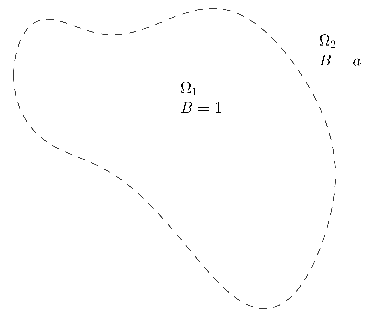
\includegraphics{fournais-et-al_fig-complete.pdf}
\caption{The plane $\mathbb R^2=\Omega_1\cup\Omega_2\cup\Gamma$ with the edge $\Gamma=\partial\Omega_1$ dashed.}\label{fig1}
\end{figure*}

The operator $\cP^a_h$ is self-adjoint in $L^2(\mathbb R^2)$ with domain
\begin{equation}\label{eq:DomP}
\textsf{ Dom}(\cP^a_{h})=\{u\in L^2(\mathbb R^2)\sep (-ih\nabla+\A)^{j}u\in L^2(\mathbb R^2),\;j=1,2\}.
\end{equation}
Its essential spectrum is determined by the magnetic field at infinity (in our case it is equal to $a$). More precisely, by Persson's lemma, we have
\[
\inf\sp_\ess(\cP^a_h)\geq |a| h.
\]
The purpose of this paper is to study the spectrum of $\cP^a_h$ in the energy window
$J_h=[0, Eh]$ with $E\in(0,|a|)$ a fixed constant (thus, we analyze the spectrum below the essential spectrum) and in the semiclassical limit $h\to 0$.
We denote by $\lambda_n(\cP^a_h)$ the $n$'th eigenvalue of $\cP^a_h$, and have
\begin{align}
\sp(\cP^a_h) \cap [0, Eh] = \{ \lambda_n(\cP^a_h) \}_{n=1}^N,
\end{align}
with $N=N(h)$.

Let us stress that our spectral analysis will be uniform with respect to $a\in[-1,a_0]$ and that the condition on the sign of $a$ is crucial since we will see that it implies a localization of the eigenfunctions associated with eigenvalues in $J_h$ near the edge $\Gamma$. That is why we will say that the edge is attractive.

\Subsection{Heuristics, earlier results, and motivation}
\subsubsection{Analogy with an electric well and mini-wells}
The problem investigated in this paper shares common features with the semiclassical asymptotics of the Schrödinger operator, $-h^2\Delta+V$, with an electric potential $V$, in the full plane, see \cite{HeSj,HeSj5,Simon, HS6}. In this context, the \enquote{well} is the set $\Gamma_V:=\{x\in\mathbb R^2\sep V(x)=\min_{\mathbb R^2} V\}$, which attracts the bound states in the limit $h\to0$. The well is said to be \emph{non-degenerate} if $\Gamma_V$ is a regular manifold, in which case the bound states might be localized near some points of $\Gamma_V$, the \emph{mini-wells}. This phenomenon of mini-wells is a manifestation of a multi-scale localization of the bound states. Interestingly, this phenomenon occurs also in the setting of the magnetic Laplacian, with a Neumann boundary condition, or with a magnetic field having a step-discontinuity as in the present article. In particular, if we consider the Neumann Laplacian with a constant magnetic field in a bounded, smooth domain, the boundary of the domain acts as the \enquote{well}
and the set of points of the boundary with maximum curvature acts as the \enquote{mini-well} (see \cite{HM01,FH06}).

\subsubsection{Some known results}
Recently in \cite{AHK, AK20}, the operator $\cP^a_h$ was considered in $L^2(\Omega)$ with Dirichlet boundary condition on $\partial \Omega$, $\Omega_1\subset \Omega$ and $\Gamma$ a smooth curve that meets $\partial\Omega$ transversely. The edge $\Gamma$ acts as the ``well'' and the set of points of $\Gamma$ with maximum curvature acts as the ``mini-well''.
Moreover, when the curvature has a unique non-degenerate maximum along the edge $\Gamma$, an accurate eigenvalue asymptotics displaying the splitting of the individual eigenvalues of $\cP^a_h$ has been derived in \cite[Th.\,1.2]{AHK}, when $-1<a<0$. This result is clearly reminiscent of \cite{FH06}.

\subsubsection{Motivation}
In the present article, we propose another perspective on the problem. Our spectral analysis will be uniform in various ways. Firstly, it will allow to derive, given some $E\in(0,|a|)$, an effective operator in the whole energy window $J_h=[0,Eh]$ with $h\in (0,h_0]$. In particular, the same strategy will provide us with Weyl estimates (estimating the number of eigenvalues in $J_h$) and the behavior of the individual eigenvalues. Secondly, it will also be uniform with respect to the parameter $a\in[-1,a_0]$. This uniformity is the key to the understanding of the transition between the regimes $a\in(-1,0)$ and $a=-1$. This is all the more motivating since the mini-well phenomenon does not occur when $a=-1$. It is indeed rather satisfactory to have a point of view encompassing quite different phenomena and showing their unity.

\subsection{The band functions}
The statement of our main results involves a family of 1D Schrödinger operators and their lowest eigenvalues, namely
the operators obtained when the magnetic step is along a straight line, in which case a dimensional reduction is possible.
This family has been the object of recent works (see \cite{AK20, HPRS16}). Let us briefly recall some of its basic properties.
Straightening the edge $\Gamma$ locally, it is natural to consider the following \enquote{tangent} operator on $\R^2$ with magnetic field
\[
B=\curl\A=\mathbf 1_{\mathbb R_+\times\mathbb R }+a\mathbf 1_{\mathbb R_-\times\mathbb R},
\]
where $ a\in[-1,a_0]$ is a fixed constant.\footnote{Our investigation concerns the attractive magnetic edge, which is the case when $a<0$. In~the opposite case, $a \in (0,1)$, the magnetic edge will no longer attract the bound states, since $\mu_a(\sigma)$ (defined in \eqref{eq:defmua}) becomes a monotone decreasing function with $\inf_{\sigma \in{\mathbb R}} \mu_a(\sigma) = a$.} This operator is explicitly given by
\begin{equation}\label{eq.Ptgt}
\cP^{\mathrm{tgt}}_h=h^2D_t^2+(hD_s-tb_a(t))^2,\quad b_a(t)=\mathbf{1}_{\mathbb R_+}(t)+a\mathbf{1}_{\mathbb R_-}(t).
\end{equation}
By using a rescaling and a partial Fourier transformation along the straight edge $t=0$, we are led to consider the analytic family of Schrödinger operators
\begin{equation}\label{eq:ha}
\mathfrak h_a[\sigma]=-\partial^2_t+\bigl(\sigma-b_a(t)t\bigr)^2,
\end{equation}
with domain
\begin{equation}\label{eq:b2}
B^2(\R)=\{u\in L^2(\R) \sep u''\in L^2(\R),\,t^2u\in L^2(\R)\},
\end{equation}
where $\sigma\in\mathbb R$ is a parameter. \\
The operator $\mathfrak h_a[\sigma]$ is self-adjoint in $L^2(\R)$ and has compact resolvent. We denote by $(\mu^{[n]}_{a}(\sigma))_{n\geq 1}$ the non-decreasing sequence of the eigenvalues (repeated according to their multiplicity) of $\mathfrak h_a[\sigma]$. For shortness, we let
\begin{align}\label{eq:defmua}
\mu_a(\sigma)=\mu^{[1]}_{a}(\sigma) = \inf \sp(\mathfrak h_a[\sigma]).
\end{align}

By the Sturm-Liouville theory, we have the following proposition.

\begin{proposition}\label{lem.simple}
All the eigenvalues of $\mathfrak h_a[\sigma]$ are simple. 
The eigenfunction associated with $\mu^{[n]}_{a}(\sigma)$ has exactly $n-1$ simple zeroes on $\R$.
\end{proposition}

The functions $\mu^{[n]}_{a}(\sigma)$, are called the band functions. When $a=1$, we are reduced to the harmonic oscillator and $\mu^{[n]}_a(\sigma)=2n-1$. When $-1\leq a<1$, the functions $\mu^{[n]}_a(\sigma)$ are no more constant functions, see \cite{HPRS16}. The lowest band function, $\mu_{a}(\sigma)$ is studied in \cite{AK20}.

\begin{proposition}[\cite{AK20, HPRS16}]\label{prop.mu-a}
For all $n\geq 1$, the function $\mu^{[n]}_{a}$ is analytic as a function of $\sigma$. Moreover, the lowest band function satisfies
\begin{equation}\label{eq:limit-mu-a}
\lim\limits_{\sigma\to-\infty}\mu_a(\sigma)=+\infty,\quad \lim\limits_{\sigma\to+\infty}\mu_a(\sigma)=|a|,
\end{equation}
and $\mu_a$ has a unique critical point, which is a non-degenerate minimum $\beta_a\in(0,|a|)$, attained at $\sigma(a)>0$.
\end{proposition}
In light of Proposition~\ref{prop.mu-a}, we write, for $E\in(0,|a|)$,
\begin{equation}\label{eq:xi-pm}
\mu^{-1}_a([\beta_a,E])=\bigl[\sigma_-(a,E),\sigma_+(a,E)\bigr],
\end{equation}
where $-\infty<\sigma_-(a,E)<\sigma(a)<\sigma_+(a,E)<+\infty$.

\subsection{Main results}
Our analysis will reveal that the semiclassical spectral asymptotics of $\cP^a_h$ in the interval $[0,Eh]$ is governed by that of an effective operator acting on the edge $\Gamma$. In particular, we obtain accurate asymptotics for the low-lying eigenvalues of $\cP^a_h$ highlighting a significant difference between the cases where $-1<a<0$ and $a=-1$.

\begin{theorem}[Case $-1<a<0$]\label{corol.a>-1}
Assume that $k$ has a unique maximum, which is non-degenerate:
\[
k_{\max}:=\max_\Gamma k=k(s_{\max}),\quad k''(s_{\max})<0.
\]
For all $a\in(-1,0)$, there exists $C(a)>0$ such that, for all $n\geq 1$,
\[
\lambda_n(\cP^a_h)=
\beta_a h-C(a)k_{\max}h^{\sfrac32}+\Bigl(n-\frac 12\Bigr)h^{\sfrac74}\sqrt{-C(a)\mu''_a(\sigma(a))k''(s_{\max})}+o_n(h^{\sfrac74}).
\] 
\end{theorem}

\skpt
\begin{remark}
\begin{enumerate}
\item Theorem~\ref{corol.a>-1} recovers the asymptotics obtained in \cite{AHK}.
The constant is given by $C(a)= -M_3(a)>0$, with $M_3(a)$ defined in \eqref{eq:moments} and calculated in \eqref{eq:m3*}.
\item The asymptotics in Theorem~\ref{corol.a>-1} is consistent with the phenomenon observed in surface superconductivity (see \cite{FH06} and references therein) and the semiclassical analysis for the Schrödinger operator with a degenerate well in \cite{HeSj5}. In this comparison, the well corresponds here to $\Gamma$ and the mini-wells correspond to the points of maximal curvature.
\item Actually, the proof of Theorem~\ref{corol.a>-1} provides us with a uniform description of the spectrum in $[0,Eh]$ and could also help determining the behavior of the eigenvalues close to $Eh$ when $E$ is non-critical for $\mu_a$, \ie when $E\neq \beta_a$. In the context of the Robin Laplacian, such considerations are the object of the ongoing work \cite{FLTRVN22}. Note also that there are some results
high up in the spectrum in the recent work \cite{GV}, where Dirichlet conditions are considered.
\item It might happen that $k$ does not have a unique minimum and even that $\Gamma$ has some symmetry properties. In this case, tunneling occurs and the eigenvalue splitting is exponentially small (see \cite{FHK22}). The proof is similar to the case of the Laplacian with a constant magnetic field and Neumann boundary condition in a symmetric domain~\cite{BHR22}.
\end{enumerate}
\end{remark}

When $a=-1$, we will prove that $C(a)=0$ and thus the second and third terms in the asymptotics formally vanish. We still get accurate estimates for the low-lying eigenvalues
of $\cP^a_h$ when $a=-1$, which involves an operator on the edge $\Gamma\simeq [-L,L)$, whose half-length is denoted by $L$.

\begin{theorem}[Case $a=-1$]\label{corol.a=-1} There exists $C_0<0$ such that, for every $n\in\N$, we have as $h\to0$,
\[
\lambda_n(\cP_h^{ \{a=-1\}})=
\beta_{-1} h+h^2\gamma_n(h)+o_n(h^2),
\]
where $\gamma_n(h)$ is the non-decreasing sequence of the eigenvalues of the differential operator
\[
\frac{\mu''_{-1}(\sigma(-1))}{2}\left(D_s+\alpha_h\right)^2+C_0k(s)^2,\quad\mbox{ with } D_s=-i\partial_s,
\] 
acting on $[-L,L)$ with periodic boundary conditions, and
\begin{equation}\label{defalphah}
\alpha_h:= \frac{|\Omega_1|}{2Lh} - \frac{\sigma(-1)}{\sqrt{h}}.
\end{equation}
Here $|\Omega_1|$ is the area of $\Omega_1$.
\end{theorem}

The quantity $\alpha_h$ in \eqref{defalphah} involves the circulation of the magnetic potential along~$\Gamma$. In fact, by Stokes' Theorem, the circulation satisfies
\[
\frac1{|\Gamma|}\int_\Gamma \A\cdot \tau \rd s(x)=\frac1{|\Gamma|}\int_{\Omega_1} \curl\A \rd x= \frac{|\Omega_1|}{2L}.
\]

At the first glance, Theorems~\ref{corol.a>-1} and \ref{corol.a=-1} seem independent. However, they both result from the analysis of the effective operator of $\cP_h^a$ (see Theorem~\ref{thm.main} below), which provides us with an accurate spectral description for $-1\leq a<0$.

This effective operator can be described as an $\hbar$-pseudodifferential operator on~$\R$ with a $2L$-periodic symbol with respect to the space variable, and acting on $2L$\nobreakdash-periodic functions. Here and along the whole paper the parameter
\begin{equation}
\hbar:=h^{1/2}
\end{equation}
is called the \emph{effective} semiclassical parameter. Let us describe the shape of our effective operator. For a given symbol $p_\hbar(s,\sigma)\in S_{\R^2}(1)$,\footnote{that is, a smooth bounded function on $\R^2$ such that its derivatives at any order are also bounded, uniformly in $\hbar\in(0,1]$.} we consider the Weyl quantization, \ie the operator defined by
\begin{equation}\label{eq.ph-w-intro}
(\Op_\hbar^w(p_\hbar) u)(s)=\frac{1}{2\pi\hbar} \int_{\R^2} e^{i(s-\tilde s)\cdot \sigma/\hbar} p_\hbar \Bigl(\frac{s+\tilde s}{2}, \sigma\Bigr)u(\tilde s) \rd \tilde s \rd \sigma.
\end{equation}
For an introduction to pseudo-differential operators, the reader is referred for instance to \cite{Zworski}, where rigorous definitions are given and several fundamental properties are established. These operators being well defined on $\mathcal S(\mathbb R)$, they can be extended by duality as operators on $\mathcal S'(\mathbb R)$. We now underline that, if $p_{\hbar}(s+2L,\sigma)=p_{\hbar}(s,\sigma)$, then $\Op_\hbar^w(p_\hbar)$ transforms all the $2L$-periodic distributions into $2L$-periodic distributions. In fact, $\Op_\hbar^w(p_\hbar)$ also preserves the space of $2L$-periodic functions that are in $L^2_{\loc}$, denoted by $L^2_{2L}(\R)$ (see Section~\ref{s-sec.p}).

Such an induced operator will give us our effective operator and we will call it \emph{a pseudodifferential operator on the edge}, $s$ representing the coordinate on $\Gamma$ (parametrized by arc-length).

\pagebreak[2]
The main result in this article is the following.

\begin{theorem}[Spectral reduction to the edge]\label{thm.main}
There exists a self-adjoint $\hbar$\nobreakdash-pseudo\-differential operator (with symbol $p_\hbar^{\eff}\in S_{\R^2}(1)$) on the edge, whose principal symbol coincides with $\mu_a$ below $E$, such that the spectrum of $\Op^w_\hbar (p^{\eff}_\hbar)$ is discrete in $[0,E]$ for $\hbar$ in some interval $(0,\hbar_0]$.

Moreover, for all $n\in\N$ such that $\lambda_n(\cP_h^a)\in J_h=[0,Eh]$, we have as $h\to0$,
\[
\lambda_n(\cP^a_h)= h\lambda_n(\Op^w_\hbar (p^{\eff}_\hbar))+o(h^{2}),
\]
uniformly with respect to $a\in[-1,a_0]$, where $-1<a_0<0$. Here $\lambda_n(\Op^w_\hbar (p^{\eff}_\hbar))$ denotes the $n$-th eigenvalue of $\Op^w_\hbar (p^{\eff}_\hbar)$.
\end{theorem}
The discreteness of the spectrum of such an $\hbar$-pseudodifferential operator, for $\hbar$ small enough, is rather classical. Indeed, fixing $E^+\in(E,|a|)$, we shall see that the principal symbol of $p_\hbar^{\eff}$ coincides with $\mu_a$ below $E^+$ and thus, since $\mu_a$ has a unique minimum, we can consider a smooth function of $\sigma$ with compact support, denoted by~$\chi$, such that $p_\hbar^{\eff}(s,\sigma)+\chi(\sigma)\geq E^+$. Since $\Op^w_\hbar \chi$ is a compact operator on $L^2_{2L}(\R)$, we get that the essential spectra of $\Op^w_\hbar (p^{\eff}_\hbar)+\Op^w_\hbar \chi$ and $\Op^w_\hbar (p^{\eff}_\hbar)$ coincide. By~using the G\aa rding inequality, this essential spectrum is contained in $ (E,+\infty)$.

The power of Theorem~\ref{thm.main} is that it yields the two different asymptotics in Theorems~\ref{corol.a>-1}~and~\ref{corol.a=-1}. The analysis in \cite{AHK} only works for $-1<a<0$, in which case the eigenfunctions are localized near the edge point(s) of maximal curvature, while in the perfectly symmetric situation when $a=-1$, the localization near the edge is displayed via an effective operator essentially independent of $h$ (and thus the corresponding eigenfunctions are not particularly localized near specific points on the edge, even in the limit $h\to 0$).

Of course, the present statement of Theorem \ref{thm.main} is not very informative if we do not describe the effective operator (see \eqref{eq.exp.eff-symb} for the expression of $p_\hbar^{\eff}$, involving the curvature $k$ along the edge $\Gamma$, viewed as a function of the arc-length $s$). However, it~\hbox{already} gives an idea of the dimensional reduction approach using the tools developed in \cite{Keraval} and inspired by \cite{GMS91, M07}.

Besides the accurate asymptotics of the low-lying eigenvalues obtained in Theorems \ref{corol.a>-1} and \ref{corol.a=-1}, another interesting result that follows from Theorem~\ref{thm.main} is a Weyl estimate.

\begin{theorem}[Asymptotic number of edge states]\label{corol.weyl}
We have
\[
N(\cP^a_h, Eh)\underset{\hbar\to 0}\sim \frac{L(\sigma_+(a,E)-\sigma_-(a,E))}{\pi\sqrt{h}}.
\]
\end{theorem}

The above Weyl estimate is similar to the one for the Neumann Laplacian with a magnetic field obtained by purely variational methods
not involving pseudodifferential techniques in \cite{F07, FK, KK}.

\enlargethispage{-\baselineskip}
\pagebreak[2]
\skpt
\begin{remark}
\begin{enumerate}
\item Our work does not cover the case when $\Gamma$ has corners, in which case a strategy of dimensional reduction might be inefficient (as in the case for the Neumann magnetic Laplacian on corner domains, see \cite{BN, BND06}).
\item Another interesting question is to analyze the behavior of the spectrum near the Landau level $|a|h$, where we loose the uniformity in our estimates and we can expect that another regime occurs.
\end{enumerate}
\end{remark}

\subsection{Organization}

In Section~\ref{sec:FlatEdge}, we discuss and recall some elementary properties of the model in $\R^2$ with a flat edge.
Section~\ref{sec:red} is devoted to the description of the Frenet coordinates along the edge $\Gamma$ and the reduction of our problem to the study of an operator in a neighborhood of $\Gamma$.
In Section~\ref{sec:pseudo}, we express the operator obtained in Section~\ref{sec:red} as an $\hbar$-pseudodifferential operator with operator symbol and expand this operator in powers of $\hbar$. In Section~\ref{sec:Gr}, we use a Grushin problem to construct a parametrix (that is an approximate inverse) for the operator introduced in Section~\ref{sec:red}.
In Section~\ref{sec:proofs}, we deduce accurate eigenvalue estimates from the Grushin reduction, finish the proof of Theorem~\ref{thm.main}, and show how it yields the other theorems announced in the introduction.

\section{The flat edge model}\label{sec:FlatEdge}
This section is devoted to the study of the flat edge model \eqref{eq.Ptgt} and more precisely to the properties of the fibered family \eqref{eq:ha}. We recall that our analysis holds for $[-1,a_0]$, with $-1<a_0<0$.

\subsection{More on the band functions}\label{sec.chi1}
We will use the following lemma.
\begin{lemma}\label{lem.mu2}
For all $\sigma\in\R$, we have
\[
\mu_a^{[2]}(\sigma)> |a|.
\] 
\end{lemma}
\begin{proof}
Let us consider the $L^2$-normalized eigenfunction $u:=u^{[2]}_{a,\sigma}$ associated with $\mu_a^{[2]}(\sigma)$. We have
\begin{equation*}
-u''(t)+(\sigma-tb_a(t))^2u(t)=\mu_a^{[2]}(\sigma) u(t).
\end{equation*}
By the Sturm-Liouville theory, $u$ has exactly one simple zero $t_0$. Assume first that $t_0\geq 0$. Then, for all $t\geq 0$,
\[
-u''(t+t_0)+(\sigma-(t+t_0))^2u(t+t_0)=\mu_a^{[2]}(\sigma) u(t+t_0).
\]
The (non-zero) function $v=u(\cdot+t_0)$ is an eigenfunction of the Dirichlet realization on $\R_+$ of $-\partial_t^2+(\sigma-t_0-t)^2$. Since $v$ does not vanish on $\R_+$, we have $\mu_a^{[2]}(\sigma)=\mu^{\Dir}_1(\sigma-t_0)>1\geq |a|$.
Now, assume that $t_0<0$. Then, for all $t\leq 0$,
\[
-u''(t+t_0)+(\sigma-a(t+t_0))^2u(t+t_0)=\mu_a^{[2]}(\sigma) u(t+t_0).
\]
In the same way, we infer that $\mu_a^{[2]}(\sigma)>|a|$.
\end{proof}

For later use, we can consider a smooth bounded increasing function $\chi_1$ on $\R$ such that $\chi_1(\sigma)=\sigma$ on a neighborhood of the interval $[\sigma_-(a,E^+),\sigma_+(a,E^+)\bigr]$, see \eqref{eq:xi-pm}. In particular $\mu_a\circ\chi_1$ has still a unique minimum at $\sigma_a$, which is not degenerate and not attained at infinity (since $\liminf_{|\sigma| \rightarrow +\infty} \mu_a (\chi_1(\sigma))> \mu_a(\sigma_a)$).
The functions $\overset{\circ}{\mu}^{[n]}_a=\mu^{[n]}_a\circ\chi_1$ will serve as bounded versions of $\mu^{[n]}_a$. We denote by $\overset{\circ}{u}_\sigma$ the positive and normalized ground state of
\begin{equation}\label{eq:circ-n}
\overset{\circ}{n}_0(\sigma):=\mathfrak h_a[\chi_1(\sigma)],
\end{equation}
where $\mathfrak h_a$ is defined in \eqref{eq:ha}.

We can express the projection on $\Span(\overset{\circ}{u}_\sigma)$ as $ \Pi^*(\sigma)\Pi(\sigma)$ where
\[
\Pi(\sigma)=\langle\cdot,\overset{\circ}{u}_{\sigma}\rangle\quad\text{and}\quad \Pi^*(\sigma)={}\cdot\, \overset{\circ}{u}_{\sigma},
\]
where we emphasize that $\Pi^*(\sigma)\in\mathcal L (\mathbb C, L^2(\mathbb R))$.
Thanks to Lemma \ref{lem.mu2} (and the spectral theorem), for all $z\in [0,E^+]$, we can consider the regularized resolvent\footnote{Since $[0,|a|)\cap\sp(\overset{\circ}{n}_0(\sigma))=\{\mu_a^{[1]}(\sigma)\}$, $\overset{\circ}{n}_0(\sigma)-z$ can be inverted on the orthogonal complement of $\overset{\circ}{u}_\sigma$, for $0\leq z<E_+<|a|$.}
\[
\overset{\circ}{\mathfrak R}_{0,z}(\sigma)= (\overset{\circ}{n}_0(\sigma)-z)^{-1}\,\bigl(\Id-\Pi^*(\sigma)\Pi(\sigma)\bigr).
\]

\begin{example}
As mentioned in the introduction, we will work with pseudodifferential operators in the $s$-variable (parallel to the boundary).
A key example is given by $\Pi$ above. We view $(s,\sigma) \mto \Pi(\sigma) \in \mathscr{L}(L^2(\R),\C)$ as an operator-valued symbol.
Thereby we get, using the Weyl quantization of \eqref{eq.ph-w-intro} in the introduction, for $\varphi=\varphi(s,t)$,
\begin{align*}
(\Op_\hbar^w(\Pi) \varphi)(s)&=\frac{1}{2\pi\hbar} \int_{\R^2} e^{i(s-\tilde s)\cdot \sigma/\hbar} (\Pi(\sigma) \varphi)(\tilde s) \rd \tilde s \rd \sigma \\
&= \frac{1}{2\pi\hbar} \int_{\R^2} e^{i(s-\tilde s)\cdot \sigma/\hbar} \int_{\R} \varphi(\tilde s,t) \overline{\overset{\circ}{u}_\sigma(t)} \rd t \rd \tilde s \rd \sigma.
\end{align*}
Similarly, $(s,\sigma) \!\mto\! \Pi(\sigma)^{*} \!\in\! \mathscr{L}(\C,L^2(\R))$ is an operator-valued symbol and for \hbox{$\psi\!=\!\psi(s)$}, we have\vspace*{-3pt}
\begin{align*}
(\Op_\hbar^w(\Pi^{*}) \psi)(s,t)
&= \frac{1}{2\pi\hbar} \int_{\R^2} e^{i(s-\tilde s)\cdot \sigma/\hbar}\psi(\tilde s) \overset{\circ}{u}_\sigma(t) \rd \tilde s \rd \sigma.
\end{align*}
\end{example}

\begin{proposition}\label{prop.Grushin0}
For all $ z\in [0,E^+]$ (or more generally $\Re z\leq E^+$), the matrix operator
\[
\mathscr{P}_{0,z}(\sigma)=\begin{pmatrix}
\overset{\circ}{n}_0(\sigma)-z&\Pi^*(\sigma)\\
\Pi(\sigma)&0
\end{pmatrix} : B^2(\R)\times\C\to L^2(\R)\times\C
\]
is bijective for all $\sigma\in\R$ and
\[
\mathscr{P}_{0,z}(\sigma)^{-1}=\begin{pmatrix}
\overset{\circ}{\mathfrak R}_{0,z}(\sigma)&\Pi^*\\
\Pi&z-\overset{\circ}{\mu}^{[1]}_a(\sigma)
\end{pmatrix}=:\mathscr{Q}_{0,z}(\sigma).
\]
Moreover, the operator symbols $(s,\sigma) \mto \mathscr{P}_{0,z}(\sigma)$ and $(s,\sigma) \mto \mathscr{Q}_{0,z}(\sigma)$ belong to $S\bigl(\R^2,\mathscr{L}(B^2(\R)\times\C, L^2(\R)\times\C)\bigr)$ and $
S\bigl(\R^2,\mathscr{L}(L^2(\R)\times\C, B^2(\R)\times\C)\bigr)$, respectively.
\end{proposition}
We recall that $S(\R^2,F)$ is the set of smooth functions on $\R^2$, valued in $F$ with bounded derivatives (at any order).

\begin{proof}
By straightforward computations, we can verify the identities
\begin{equation*}
\mathscr Q_{0,z}(\sigma)\mathscr P_{0,z}(\sigma)=\Id_{B^2(\R)\times \C} \mbox{ and } \mathscr P_{0,z}(\sigma)\mathscr Q_{0,z}(\sigma)=\Id_{L^2(\R)\times\C}.\qedhere
\end{equation*}
\end{proof}

\subsection{Some useful formulas}\label{sec:uf}
Let us recall some formulas and results from \cite{AK20}. Let $\phi_a$ be the \emph{positive} and $L^2$-normalized ground state of the operator $\overset{\circ}{n}_0(\sigma(a))$. introduced in \eqref{eq:circ-n}. It is proved in \cite[Th.\,1.1]{AK20} that $\phi_a'(0)<0$ for all $a\in(-1,a_0)$.

Some useful identities involve the moments
\begin{equation}\label{eq:moments}
M_n(a)=\int_{\mathbb R}\frac 1{b_a(\tau)}\bigl(b_a(\tau)\tau-\sigma(a)\bigr)^n|\phi_a(\tau)|^2\,d\tau, \end{equation}
for $n\in \mathbb N $.
It has been proved in \cite{AK20} that
\begin{align}
M_1(a)&=0,\label{eq:m1}\\
M_2(a)&=-\frac 12 \beta_a\int_{\mathbb R}\frac 1{b_a(\tau)}|\phi_a(\tau)|^2\,d\tau+\frac 14\Bigl(\frac 1a-1\Bigr)\sigma(a)\phi_a(0)\phi_a'(0), \label{eq:m2}\\
M_3(a)&=\frac 13\Bigl(\frac 1a-1\Bigr)\sigma(a)\phi_a(0)\phi_a'(0).\label{eq:m3*}
\end{align}
The case $a=-1$ is special because
\[
M_2(-1)=M_3(-1)=0,
\]
while, for $-1<a<0$, $M_3(a)<0$.

Finally, we will also need the following two identities \cite[Rem.\,2.3]{AHK},
\begin{equation}\label{aqddid}
\begin{split}
\int_{\mathbb R}\tau(\sigma(a)-b_a(\tau) \tau)^2|\phi_a(\tau)|^2\,\rd \tau&=M_3(a) +\sigma(a)M_2(a),\\
\int_{\mathbb R}b_a(\tau) \tau^2(\sigma(a)-b_a(\tau) \tau)|\phi_a(\tau)|^2\,\rd \tau&=-M_3(a)-2\sigma(a)M_2(a).
\end{split}
\end{equation}

\subsection{The symmetric case $a=-1$ and the de\,Gennes model}\label{sec.dG}
Let us recall the definition and properties of the de\,Gennes model occurring in the analysis of surface superconductivity within the Ginzburg-Landau model \cite[\S 3.2]{FH10} (and references therein). We start with the family of harmonic oscillators
\[
\mathfrak h[\sigma]=-\partial_t^2+(\sigma-bt)^2
\]
on the half-axis $\R_+$ with Neumann condition at $0$. Let us denote the positive normalized ground state of $\mathfrak h[\sigma]$ by $f_{\sigma}$ and the ground state energy by $\mu(\sigma)$. Then, minimizing with respect to $\sigma\in\R$ we get
\[
\Theta_0=\inf_{\sigma\in\R}\mu(\sigma)=\mu(\xi_0),\quad\text{where~}\xi_0=\sqrt{\Theta_0}.
\]
Let $f_0:=f_{\xi_0}$. Then, for $a=-1$, we get by a symmetry argument
\[
\phi_a(t)=f_0(|t|)\,
\quad \text{and}\quad \sigma(-1) = \xi_0.
\]

\subsubsection*{Moments}
Let us introduce the following moments
\[
M_k=\int_{\R_+}(\xi_0-t)^k|f_0(t)|^2\rd t.
\]
Then, by \cite{FH06}, we have
\begin{equation}\label{eq:moments3}
M_0=1,\quad M_1=0,\quad M_2=\frac{\Theta_0}2 ,\quad M_3=-\frac{|f_0(0)|^2}{6},
\end{equation}
and
\[
M_4= \frac{3}{8}\bigl(1+\Theta_0^2-\xi_0f_0(0)^2 \bigr)=\frac38(1+\Theta_0^2+6\xi_0M_3).
\]

\section{Decay of bound states and spectral reduction}\label{sec:red}

In this section, we consider the eigenfunctions of the operator $\cP^a_h=\cP_h$ with eigenvalues in the energy window
\begin{equation}
J^+_h=[0,E^+h]\quad\text{where~} E<E^+<|a|.
\end{equation}

We prove that the eigenfunctions associated with eigenvalues in $J^+_h$ are exponentially localized near $\Gamma$, see Corollary \ref{cor.expdecay}. To describe the effect of the edge on the localization, it is natural to use the classical tubular coordinates near $\Gamma$, whose definition will be recalled in Subsection \ref{sec.tubular}. In order to prove Corollary \ref{cor.expdecay},
we will have to combine Agmon estimates and a rough estimate on the number of eigenvalues in~$J^+_h$ (polynomially in $h^{-1})$), which will be discussed in Subsection \ref{sec.number}.

\subsection{Tubular coordinates}\label{sec.tubular}
For all $\epsilon>0$, consider the $\epsilon$-neighborhood of $\Gamma$
\begin{equation}\label{eq:gam-ep}
\Gamma(\epsilon)=\{x\in\mathbb R^2\sep \dist(x,\Gamma)<\epsilon\}.
\end{equation}
Consider a parameterization $\bM(s)$ of the edge $\Gamma$ by the arc-length coordinate $s\in\nobreak[-L,L)$, where $L=|\Gamma|/2$. Consider the unit normal $\bn(s)$ to $\Gamma$ pointing inward to~$\Omega_1$, and the unit oriented tangent $\bt(s)=\dot{\bn}(s)$ so that $(\bt(s),\bn(s))$ is a direct frame, \ie $\det(\bt(s),\bn(s))=1$. We can now introduce the curvature $k(s)$ at the point $\bM(s)$, defined by $\ddot{\bn}(s)=k(s)\bn(s)$.

Let us represent the torus $(\mathbb R/ 2L \mathbb Z)$ by the interval $[-L,L)$ and pick $\epsilon_0>0$ so that
\[
\Phi: \mathbb R/ (2L \mathbb Z)\times (-\epsilon_0,\epsilon_0)\ni (s,t)\mto \bM(s)+t\bn(s)\in\Gamma(\epsilon_0)
\]
is a diffeomorphism, with Jacobian
\begin{equation}\label{defm}m(s,t)=1-tk(s).
\end{equation}
The Hilbert space $L^2(\Gamma(\epsilon_0))$ is transformed into the weighted space
\[
L^2\bigl((\mathbb R/ 2L \mathbb Z) \times(-\epsilon_0,\epsilon_0);m\,\rd s\rd t\bigr)
\] and the operator $\cP_h$ is (locally near the edge) transformed into the following operator (see \cite[App.\,F]{FH10})):
\begin{multline*}
\widetilde{\cP}_h:=-h^2m^{-1}\partial_t m\partial_t\\+m^{-1}\Bigl(-ih\partial_s+\gamma_0-b_a(t)t+\frac{k}{2}b_a(t)t^2\Bigr)m^{-1}\Bigl(-ih\partial_s+\gamma_0-b_a(t)t+\frac{k}{2}b_a(t)t^2\Bigr),
\end{multline*}
where $b_a$ is defined in \eqref{eq:ha} and
\begin{equation}\label{eq:circ}
\gamma_0=\frac{|\Omega_1|}{2L}.
\end{equation}
\subsection{Number of eigenvalues}\label{sec.number}
We give a preliminary, rough bound on
the number of eigenvalues in $J^+_h$. As we will see, this first estimate will be enough to deduce a stronger one at the end of our analysis.
\begin{proposition}\label{prop:Nb-h}
Let $N(\cP_h, E^+h)=\Tr\bigl(\mathbf 1_{J_h}(\cP_h)\bigr)$. There exist $C,h_0>0$ such that, for all $h\in(0,h_0)$,
\[
N(\cP_h, E^+h)\leq C h^{-2}.
\]
\end{proposition}
\begin{proof}
Let us introduce a fixed partition of the unity
\[
\chi_{\out}^2+\chi_{\rme}^2+\chi_{\rin}^2=1,
\] 
such that $\supp(\chi_{\out})\subset\mathbb{R}^2\setminus\overline{\Omega}_1=\Omega_2$, $\supp(\chi_{\rin})\subset\Omega_1$, and ${\supp(\chi_{\rme})}\subset \overline{\Gamma(\epsilon_0)}$.
The quadratic form associated with $\cP_h$ is given by 
\[
Q_h(\psi)=\int_{\R^2}|(-ih\nabla+\A)\psi|^2\rd x,
\]
for all $\psi\in L^2(\R^2)$ such that $(-ih\nabla+\A)\psi\in L^2(\R^2)$.

The usual localization formula (see, for instance, \cite[\S 4.1.1]{Ray}) gives the existence of a constant $C>0$ such that
\[
Q_h(\psi)\geq Q_h(\chi_{\out}\psi)+Q_h(\chi_{\rme}\psi)+Q_h(\chi_{\rin}\psi)-Ch^2\|\psi\|^2.
\]
By noticing that $\psi\mto(\chi_{\out}\psi,\chi_{\rme}\psi,\chi_{\rin}\psi)$ is injective, and thanks to the min-max theorem, we find that
\[
N(\cP_h, E^+h)\leq N(\cP^{\out}_h,E^+h+Ch^2)+N(\cP_h^{\rme},E^+h+Ch^2)+N(\cP_h^{\rin},E^+h+Ch^2),
\]
where the operators $\cP^{\out}_h$, $\cP^{\rme}_h$ and $\cP^{\rin}_h$ are the Dirichlet realizations of $(-ih\nabla+\A)^2$ on $\Omega_2$, $\Gamma(\epsilon_0)$ and $\Omega_1$, respectively.
We recall that $E^+<|a|\leq |a_0|<1$ and notice that $\cP^{\out}_h\geq |a|h$ and $\cP^{\rin}_h\geq h$. When $h$ is small enough, $E^+h+Ch^2<|a|h<h$, so we must have $N(\cP^{\out}_h,E^+h+Ch^2)=N(\cP^{\rin}_h,E^+h+Ch^2)=0$. Thus,
\[
N(\cP_h, E^+h)\leq N(\cP_h^{\rme},E^+h+Ch^2).
\]
Therefore, we are reduced to estimate the number of eigenvalues of the operator with compact resolvent $\cP_h^{\rme}$ below $E^+h+Ch^2$. For that purpose, we can use the tubular coordinates and notice that, for all $\psi\in H^1_0(\Gamma(\epsilon_0))$,
\[
Q_h(\psi)=\int_{(\mathbb R/ 2L \mathbb Z)\times(-\epsilon_0,\epsilon_0)}\Bigl(|h\partial_t\psi|^2+m^{-2}|(hD_s+\gamma_0-b_a(t)t+\frac{k}{2}t^2)\psi|^2\Bigr)m\rd s\rd t.
\]
This gives the following rough estimate, for some $c_0,C_0>0$,
\[
\frac{Q_h(\psi)}{\|\psi\|^2}\geq c_0\frac{\int_{(\mathbb R/ 2L \mathbb Z)\times(-\epsilon_0,\epsilon_0)} |h\partial_t\psi|^2+|h\partial_s\psi|^2\rd s\rd t}{\int_{(\mathbb R/ 2L \mathbb Z)\times(-\epsilon_0,\epsilon_0)} |\psi|^2\rd s\rd t}-C_0.
\]
Thanks to the min-max theorem, this implies the upper bound
\[
N(\cP_h^{\rme},E^+h+Ch^2)\leq N(-h^2\Delta^{\Dir},c_0^{-1}(E^+h+Ch^2+C_0)),
\]
where $-\Delta^{\Dir}$ is the Dirichlet Laplacian on the cylinder $(\mathbb R/ 2L \mathbb Z)\times(-\epsilon_0,\epsilon_0)$. The spectrum of this operator can be computed explicit thanks to Fourier series, and we get the rough estimate
\[
N(-h^2\Delta^{\Dir},c_0^{-1}(E^+h+Ch^2+C_0))\leq\tilde Ch^{-2}.\qedhere
\]
\end{proof}

Since $E^+<|a|$, the eigenfunctions of $\cP_h$ associated with eigenvalues in the allowed energy window $J^+_h$ are localized near the edge, see \cite{AK20}.

\begin{proposition}\label{prop:dec}
There exist constants $\alpha,h_0,C_0>0$ such that, if $h\in (0,h_0]$ and~$u_h$ is an eigenfunction of $\cP_h$ associated with an eigenvalue in $J^+_h$, then the following holds,
\begin{equation}\label{eq:dec-norm}
\int_{\mathbb R^2}\bigl(|u_{h}|^2+h^{-1}|(-ih\nabla+\A)u_{h}|^2 \bigr)\exp\Bigl(\frac{2\alpha\dist(x,\Gamma)}{h^{1/2}} \Bigr)\rd x\leq C_0\|u_h\|^2_{L^2(\R^2)}.
\end{equation}
\end{proposition}

Combining Propositions \ref{prop:Nb-h} and \ref{prop:dec}, we get the following estimate.
\begin{corollary}\label{cor.expdecay}
Let $\eta\in\left(0,\sfrac12\right)$. There exists $h_0>0$ such that for all $h\in(0,h_0)$ and $u_h\in \dist\mathds{1}_{J_h}(\cP_h)$, we have outside $\Gamma(h^{\sfrac12-\eta})$
\begin{equation}\label{eq:dec-norm'}
\int_{\mathbb{R}^2\setminus\Gamma(h^{\sfrac12-\eta})}\bigl(|u_{h}|^2+|(-ih\nabla+\A)u_{h}|^2 \bigr)\rd x\leq e^{-h^{-\eta}}\|u_h\|^2_{L^2(\R^2)}.
\end{equation}
\end{corollary}

Corollary \ref{cor.expdecay} suggests to use the rescaling $t=\hbar \tilde t$. We also consider a smooth cutoff function
\begin{equation}\label{eq:c-delta}
c_\mu(\tilde t)= c(\mu\tilde t),\quad \mu=h^{\eta}=\hbar^{2\eta},
\end{equation}
where $c\in \mathscr{C}^\infty_0(\mathbb R)$ is even and satisfies $c=1$ on $[-1,1]$ and $c=0$ on $\mathbb R\setminus(-2,2)$. This cutoff function is convenient to define the new operator on the Hilbert space\break$ L^2\bigl((\mathbb R/ 2L \mathbb Z)\times\mathbb R;m_\hbar \rd \tilde s \rd \tilde t\bigr)$, by
\begin{multline*}
\widetilde{\mathcal N}_{\hbar}=-m^{-1}_{\hbar}\partial_{\tilde t} m_{\hbar}\partial_{\tilde t}\\
+m^{-1}_{\hbar}\Bigl(\hbar D_{\tilde s}+\hbar^{-1}\gamma_0-b_a\tilde t +\hbar c_\mu \,\frac{k}{2}\,b_a\tilde t^2\Bigr) m^{-1}_{\hbar}\Bigl(\hbar D_{\tilde s}+\hbar^{-1}\gamma_0-b_a\tilde t+\hbar c_\mu\,\frac{k}{2}\,b_a\tilde t^2\Bigr)
\end{multline*}
acting on the domain
\begin{multline*}
\Dom(\widetilde{\mathcal N}_{\hbar})=\bigl\{ u\in L^2\bigl((\mathbb R/ 2L \mathbb Z)\times\mathbb R\bigr)\sep \partial_{\tilde t}^2u\in L^2\bigl((\R/2L\Z)\times\mathbb R\bigr), \\
(\hbar D_{\tilde s}+\hbar^{-1}\gamma_0-b_a\tilde t)^2 u \in L^2\bigl((\mathbb R/ 2L \mathbb Z)\times\mathbb R\bigr) \bigr\}.
\end{multline*}
As in Proposition \ref{prop:dec}, we can prove that the eigenfunctions of $\widetilde{\mathcal{N}}_h$ associated with eigenvalues in $J_h$ are localized near $\tilde t=0$.

\begin{proposition}
\label{prop:BHR2.7}
The spectra of $\cP_h$ and $\widetilde{\mathcal{N}}_h$ in $J^+_h$ coincide modulo $\mathcal{O}(h^{\infty})$.
\end{proposition}

Therefore, we are reduced to the spectral analysis of $\widetilde{\mathcal{N}}_h$. For shortness, we drop the tildes. Up to a change of gauge, we are reduced to the operator\vspace*{-3pt}
\begin{multline*}\label{eq:tilde-Nh}
{\mathcal N}_{\hbar,\theta}=-m^{-1}_{\hbar}\partial_{t} m_{\hbar}\partial_{t}\\[
-3pt]
+m^{-1}_{\hbar}\Bigl(\hbar D_{ s}+\theta-b_a t +\hbar c_\mu \frac{k}{2}b_a t^2\Bigr) m^{-1}_{\hbar}\Bigl(\hbar D_{ s}+\theta-b_a t+\hbar c_\mu\,\frac{k}{2}\,b_a t^2\Bigr),
\end{multline*}
with\vspace*{-3pt}
\[
m_\hbar (\tilde s,\tilde t):= 1- \hbar c_\mu(\tilde s,\tilde t) \tilde t k(\tilde s),
\]
and domain\vspace*{-3pt}
\begin{multline*}
\Dom({\mathcal N}_{\hbar,\theta})=\{ u\in L^2\bigl((\mathbb R/ 2L \mathbb Z)\times\mathbb R)\sep \partial_{t}^2u\in L^2((\R/2L\Z)\times\mathbb R\bigr), \\
(\hbar D_{s}+\theta-b_a t)^2 u \in L^2(((\mathbb R/ 2L \mathbb Z))\times\mathbb R) \}.
\end{multline*}
Here\vspace*{-3pt}
\begin{subequations}
\begin{equation}\label{eq:defthetaa}
\theta=\theta(\hbar)=\hbar^{-1}\gamma_0-\frac{m\pi}{L}\hbar,
\end{equation}
where $m\in\Z$ is chosen so that\vspace*{-3pt}
\begin{equation}\label{eq:defthetb}
\theta(\hbar)\in[0,\hbar\pi L^{-1}).
\end{equation}
\end{subequations}

Before going ahead, we have to deal with the inconvenience of working in a Hilbert space with a weighted measure, which also depends on $\hbar$. Thus, let us use the canonical conjugation and work in the fixed Hilbert space with flat measure
\hbox{$L^2((\R/2L\Z)\times\R,\rd s\rd t)$}:
\begin{equation}\label{eq:Nhc0}
\begin{aligned}
\mathfrak N_{\hbar,\theta}&=m_\hbar^{1/2}\mathcal N_{\hbar,\theta}m_\hbar^{-1/2}=-m^{-1/2}_{\hbar}\partial_t m_{\hbar}\partial_t m_{\hbar}^{-1/2}+\bigl(m_\hbar^{-1/2} \mathcal T_\hbar m_\hbar^{-1/2}\bigr)^2,
\end{aligned}
\end{equation}
where\vspace*{-3pt}
\begin{equation}\label{eq.Th}
\mathcal T_{\hbar,\theta}= \hbar D_s+\theta-b_at+\hbar c_\mu\,\frac{k}{2}\,b_at^2.
\end{equation}
Note that\vspace*{-3pt}
\begin{equation}\label{eq.transverse}
-m^{-1/2}_{\hbar}\partial_t m_{\hbar}\partial_t m_{\hbar}^{-1/2}=-\partial^2_t-\frac{(\partial_tm_\hbar)^2}{4m^2_\hbar}+\frac{\partial^2_tm_\hbar}{2m_\hbar},
\end{equation}
so that\vspace*{-3pt}
\begin{equation}\label{eq:Nhc}
\mathfrak N_{\hbar,\theta}=-\partial^2_t-\frac{(\partial_tm_\hbar)^2}{4m^2_\hbar}+\frac{\partial^2_tm_\hbar}{2m_\hbar}+\bigl(m_\hbar^{-1/2} \mathcal T_{\hbar,\theta} m_\hbar^{-1/2}\bigr)^2.
\end{equation}

We restate the Proposition~\ref{prop:BHR2.7} in terms of the new notation.
\begin{proposition}\label{prop:BHR2.7-bis}
The spectra of $\cP_h$ and $\mathfrak N_{\hbar,\theta}$ in $J^+_h$ coincide modulo $\mathcal{O}(h^{\infty})$.
\end{proposition}

\section{A pseudodifferential operator with operator valued symbol}\label{sec:pseudo}

\subsection{Preliminaries}\label{s-sec.p}
Let us briefly prove that an operator given by \eqref{eq.ph-w-intro} with a $2L$ periodic symbol, $p_{\hbar}(s+2L,\sigma)=p_{\hbar}(s,\sigma)$, preserves $2L$-periodic distributions and also locally square integrable $2L$-periodic functions. More generally, it also preserves the set of functions
\begin{equation}\label{eq.Fthetah}
\mathscr{F}_{\hbar,\theta}:=\{u\in L^2_{\loc}(\mathbb{R}) \sep u(s+2L)=e^{2i\theta L/\hbar}u(s)\},
\end{equation}
equipped with the $L^2$-norm on a period $[-L,L)$. The operator $\Op_\hbar^w(p_\hbar)$ acts \hbox{continuously} on $\mathscr{F}_{\hbar,\theta}$.
In fact, this is even true in the vector valued case where we~replace $u\in L^2_{\loc}(\mathbb{R})$ by $u\in L^2_{\loc}(\mathbb{R};F)$ for some Hilbert space $F$ in the definition of~$\mathscr{F}_{\hbar,\theta}$.

Let us explain this for $\theta=0$.
From the composition theorem for pseudodifferential operators (see \cite[Th.\,4.18]{Zworski}), we see that $\langle x\rangle^{-1}\Op_\hbar^w(p_\hbar)\langle x\rangle$ is a pseudodifferential operator with symbol in $S(1)$ (and thus it is bounded on $L^2(\R)$ thanks to the Calderón-Vaillancourt theorem, see \cite[Th.\,4.23]{Zworski}). This shows that $\Op_\hbar^w(p_\hbar)$ is bounded from $L^2(\R,\langle x\rangle^{-2}\rd x)$ to $L^2(\R,\langle x\rangle^{-2}\rd x)$. Notice that there exist $C_1(L)>0$, $C_2(L)>0$ and $C_3(L)>0$ such that for all $u\in L^2_{2L}(\R)$,
\begin{multline*}
\|u\|^2_{L^2(\R,\langle x\rangle^{-2}\rd x)} \leq C_1(L) \sum_{\ell \in \mathbb Z} \langle\ell\rangle^{-2} \| u\|^2_{L^2(2 \ell L - L ,2\ell L + L)} \leq C_2(L) \|u\|^2_{L^2_{2L}(\R)}\\
\leq C_3(L)\|u\|^2_{L^2(\R,\langle x\rangle^{-2}\rd x)} .
\end{multline*}
Now the operator $\mathfrak{N}_{\hbar,\theta}$ introduced in \eqref{eq:Nhc} (with $\mathcal T_{\hbar,\theta}$ introduced in \eqref{eq.Th}) can be seen as the action of an $\hbar$-pseudodifferential operator $\mathfrak{N}_\hbar$ with operator symbol $n_{\hbar}$ on $\mathscr{F}_{\hbar,\theta(\hbar)}$ where $\theta(\hbar)$ is defined in \eqref{eq:defthetb}. We have
\begin{equation}\label{eq:N0}
\mathfrak N_{\hbar}=-\partial^2_t-\frac{(\partial_tm_\hbar)^2}{4m^2_\hbar}+\frac{\partial^2_tm_\hbar}{2m_\hbar}+\bigl(m_\hbar^{-1/2} \mathcal T_{\hbar} m_\hbar^{-1/2}\bigr)^2,
\end{equation}
with
\[
\mathcal T_{\hbar}= \hbar D_s-b_at+\hbar c_\mu\,\frac{k}{2}\,b_at^2.
\]
Note that, by using the Floquet-Bloch transform, $\mathfrak{N}_\hbar$ is unitarily equivalent to the direct integral of the $\mathfrak{N}_{\hbar,\theta}$.

We recall the classical notation for the Weyl quantization
\begin{equation}\label{eq:Nhc-symb}
\Op^w_\hbar (n_{\hbar}) u (s)=\frac{1}{(2\pi\hbar)} \int_{\mathbb R^2} e^{i(s-\tilde s)\cdot \sigma/\hbar} n_{\hbar} \Bigl(\frac{s+\tilde s}{2}, \sigma\Bigr)u(\tilde s) \rd \tilde s \rd \sigma.
\end{equation}

Let us explain why the operator $\mathfrak{N}_\hbar$ can be written under the form \eqref{eq:Nhc-symb}. Note already that, at a formal level, we expect that
\[
n_{\hbar}\simeq n_0=-\partial^2_t+(\sigma-b_a t)^2.
\]
This formal principal symbol suggests to consider a set of operator-valued symbols (containing $n_0$).
We will need to introduce the space $B_{(s,\sigma)}^2(\R)$. As a vector space we have $B_{(s,\sigma)}^2(\R) = B^2(\R)$ (as defined in \eqref{eq:b2}) and the index $(s,\sigma)$ refers to the norm, given by
\[
\|\psi\|^2_{B_{(s,\sigma)}^2(\R)}=\langle \sigma\rangle^4 \bigl(\|\partial^2_t\psi\|^2+\|\langle t^2\rangle\psi\|^2\bigr).
\]
Here we used the standard notation
\begin{equation}\label{eq:<u>}
\langle u\rangle=(1+|u|^2)^{1/2}.
\end{equation}

We denote by $S\bigl(\R^2,\mathscr{L}(B_{(s,\sigma)}^2(\R),L^2(\R))\bigr)$ the class of symbols $\Psi$ on $\mathbb R^2$
with value in $\mathscr{L}(B_{(s,\sigma)}^2(\R),L^2(\R))$, such that, for all $j,k \in \mathbb N$, there exists $C_{j,k} >0$
\[
\| \partial_s^j\partial_\sigma^k \Psi (s,\sigma)\|_{\mathscr{L} (B_{(s,\sigma)}^2(\mathbb R),L^2(\mathbb R))}\leq C_{j,k}.
\]

It is inconvenient for a pseudodifferential calculus that the norm above depends on~$\sigma$. Therefore, to have uniformity in $\sigma$ we will later introduce a localization in $\sigma$, so that $\sigma$ will essentially be bounded in all expressions.
The notation $B^2(\R)$ (without indices) will refer to the space with norm
\[
\|\psi\|^2_{B^2(\R)}=\|\partial^2_t\psi\|^2+\|\langle t^2\rangle\psi\|^2 .
\]
Similarly,
$S\bigl(\R^2,\mathscr{L}(B^2(\R),L^2(\R))\bigr)$ denotes the class of symbols $\Psi$ on $\mathbb R^2$
with value in $\mathscr{L}(B^2(\R),L^2(\R))$.

More generally, we define, for $j\in {\mathbb N}$,
\begin{equation}\label{eq:bj}
\|\psi\|^2_{B_{(s,\sigma)}^j(\R)}=\langle \sigma\rangle^{2j} \bigl(\|\partial^j_t\psi\|^2+\|\langle t^j\rangle\psi\|^2\bigr), \qquad
\|\psi\|^2_{B^j(\R)}= \|\partial^j_t\psi\|^2+\|\langle t^j\rangle\psi\|^2.
\end{equation}

Our symbols can be $\hbar$-dependent and in this case we impose above the uniformity of the constants with respect to $\hbar$.\/
The representation of $\mathfrak{N}_{\hbar}$ as a pseudo-differential operator follows from the results of composition for operator symbols (see \cite[Th.\,2.1.12]{Keraval}) and by noticing that the symbol of \eqref{eq.Th} (obtained by replacing $\hbar D_s$ by $\sigma$) belongs to $S\bigl(\R^2,\mathscr{L}(B_{(s,\sigma)}^1(\R),L^2(\R))\bigr)$ and also to $S\bigl(\R^2,\mathscr{L}(B_{(s,\sigma)}^2(\R),B_{(s,\sigma)}^1(\R))\bigr)$. Indeed, the function $t\mto\hbar b_a c_\mu t^2$ is bounded, uniformly in $\hbar$, since $\mu=\hbar^{2\eta}$ (for $\eta$ fixed small enough).

\begin{remark}
We recall that the operator and its Weyl symbol are related by the following exact formula (see for instance \cite[Th.\, 4.19 \& 4.13]{Zworski} whose proof can be adapted to operator-valued symbols):
\[
n_{\hbar}(s,\sigma)=e^{-i\Psfrac\hbar2 D_s D_\sigma} \bigl[e^{-is\sigma/\hbar}\mathfrak{N}_{\hbar} (e^{i\cdot\sigma/\hbar}) \bigr](s,\sigma),
\]
where $e^{-i\Psfrac\hbar2 D_s D_\sigma}$ is defined as a Fourier multiplier thanks to the Fourier transform with respect to $(s,\sigma)$.
\end{remark}

\subsection{Expansion of $\mathfrak{N}_{\hbar}$}
Let us now describe an expansion of $n_{\hbar}$---the symbol of~$\mathfrak{N}_{\hbar}$---in powers of $\hbar$. We would like to write
\begin{equation}\label{eq:exp-symb-Nhc}
n_{\hbar}\simeq n_0+\hbar n_1+\hbar^2n_2+\cdots
\end{equation}
With this writing, we mean an expansion of the associated operator $\mathfrak N_{\hbar}$ of the following form
\begin{equation}\label{eq:ex-Nhc}
\mathfrak{N}_{\hbar}=\mathfrak n_0+\hbar\mathfrak n_1+\hbar^2\mathfrak n_2+\mathcal \hbar^3\mathscr R_\hbar^{(3)}+\hbar w_\hbar,
\end{equation}
where, for some $N\in\mathbb {N}$, $C, \hbar_0>0$, we have, for all $\hbar\in(0,\hbar_0)$,

\begin{enumerate}
\item\label{eq.i} $w_{\hbar}$ is a smooth function supported in $\{(s,t) \sep C^{-1}\hbar^{-2\eta}\leq \langle t\rangle\leq C\hbar^{-2\eta}\}$ and such that $w_\hbar=\mathscr{O}(\langle t\rangle)$ ,
\item \label{eq.ii}$\mathscr R_\hbar^{(3)}$ is a pseudodifferential operator whose symbol belongs to a bounded set in $S(\R^2,\mathscr{L}(B_{(s,\sigma)}^2(\R),L^2(\R,\langle t\rangle^{-N}\rd t)))$.
\end{enumerate}
Note that \eqref{eq:exp-symb-Nhc} is {\it not} an expansion in the symbol class $S(\R^2,\mathscr{L}(B_{(s,\sigma)}^2(\R),L^2(\R)))$, which contains $n_{\hbar}$.
We start by expanding the differential operator $\mathfrak{N}_{\hbar}$ (see \eqref{eq:Nhc}) with respect to $\hbar$, with $\mu$ (involved in the cutoff functions $c_\mu$) considered as a parameter.\footnote{Note that $\hbar c_{\mu}(t)t$ converges to $0$ uniformly as $\hbar$ tends to $0$ since $\mu=\hbar^{2\eta}$ and $\eta<1/2$.}

In the following proposition, we describe the (symmetric) differential operators $\mathfrak{n}_j$.
\begin{proposition}
The decomposition \eqref{eq:ex-Nhc} holds with
\begin{equation}\label{eq:ex-terms}
\begin{aligned}
\mathfrak n_0&=-\partial_t^2+\mathfrak{p}_0^2,\\
\mathfrak n_1&=\mathfrak p_0\mathfrak p_1+\mathfrak p_1\mathfrak p_0,\\
\mathfrak n_2&=\mathfrak p_0\mathfrak p_2+\mathfrak p_1^2+\mathfrak p_2\mathfrak p_0-c_\mu^2\frac{k^2}{4},
\end{aligned}
\end{equation} 
where
\begin{equation}\label{eq:D-theta}
\begin{aligned}
\mathfrak{p}_0&=\hbar D_s-b_a t,\\
\mathfrak{p}_1 &=c_\mu t\Bigl(\frac{k}2\mathfrak p_0+\frac12\mathfrak p_0k+\frac{k}2\, b_at \Bigr),\\
\mathfrak{p}_2&=c_\mu^2t^2\Bigl(\frac{k^2}{2}\,\mathfrak p_0+\frac12\mathfrak p_0k^2+\frac{k^2}2\,b_at \Bigr).
\end{aligned}
\end{equation}
\end{proposition}

\begin{proof}
Let us provide a Taylor expansion of \eqref{eq:Nhc}. \eqref{eq.Th} can be rewritten in the form
\[
\mathcal T_{\hbar}= \mathfrak{p}_0+\hbar c_\mu\,\frac{k}{2}\,b_at^2.
\]
Straightforward computations yield,
\[
\begin{aligned}
m_\hbar^{-1/2}\mathcal T_{\hbar} m_\hbar^{-1/2}&=m_\hbar^{-1}\mathfrak p_0+m_\hbar^{-1/2}\bigl(\hbar D_s m_\hbar^{-1/2}\bigr)+\hbar c_\mu\,\frac{k}{2}\,b_at^2 m_\hbar^{-1}\\
&=m_\hbar^{-1}\mathfrak p_0+\hbar^2 m_\hbar^{-2} c_\mu t(D_sk)+\hbar m_\hbar^{-1}c_\mu\,\frac{k}{2}\,b_at^2 .
\end{aligned}
\]
Now we expand $m_\hbar^{-1}$ in powers of $\hbar$ and get
\[
m_\hbar^{-1}=1+\hbar c_\mu tk+\hbar^2c_\mu^2t^2k^2+\hbar^3\frac{(c_\mu t k)^3}{1-\hbar c_\mu t k},
\]
so that
\[
\begin{aligned}
\hbar^2m_\hbar^{-2}&=\hbar^2+\hbar^3\frac{2c_\mu tk}{1-\hbar c_\mu tk}+\hbar^4\frac{c_\mu^2t^2k^2}{(1-\hbar c_\mu tk)^2},\\
\quad
\hbar m_\hbar^{-1}&=\hbar+\hbar^2 c_\mu tk+\hbar^3\frac{c_\mu^2t^2k^2}{1-\hbar c_\mu t k}.
\end{aligned}
\]

We have the following expansion
\begin{multline*}
m_\hbar^{-1/2} \mathcal T_{\hbar} m_\hbar^{-1/2}= \mathfrak{p}_0+\hbar kc_\mu t\Bigl(\mathfrak p_0+\frac12 b_at \Bigr)
+\hbar^2 \Bigl(k^2c_\mu^2t^2\Bigl(\mathfrak p_0+\frac12b_at \Bigr)+
\frac12c_\mu t(D_sk) \Bigr)\\
+\frac{\mathcal \hbar^3c_\mu t k}{1-\hbar c_\mu t k} \Bigl((c_\mu t k)^2 \mathfrak p_0+\Bigl(2 +\frac{\hbar c_\mu t k }{1-\hbar c_\mu tk }\Bigr)c_\mu t(D_sk)+
\frac{2c_\mu^2 t^3k^2}{2} \Bigr).
\end{multline*}
The previous expression can be rearranged as follows
\[
m_\hbar^{-1/2} \mathcal T_{\hbar} m_\hbar^{-1/2}= \mathfrak{p}_0+\hbar \mathfrak{p}_1 +\hbar^2 \mathfrak{p}_2+\mathcal \hbar^3\mathscr R_\hbar
\]
and
\begin{multline}\label{eq.remainder}
\mathscr R_\hbar=
-\hbar c_\mu^2t^2(D_sk)k\\
+\frac{c_\mu t k}{1-\hbar c_\mu t k} \Bigl((c_\mu t k)^2 \mathfrak p_0+\Bigl(2 +\frac{\hbar c_\mu t k }{1-\hbar c_\mu tk }\Bigr)c_\mu t(D_sk)+
\frac{2c_\mu^2 t^3k^2}{2} \Bigr).
\end{multline}
Recalling \eqref{eq.transverse}, we can also expand the operator in the transversal variable and get
\begin{subequations}
\begin{equation}\label{vhwha}
-m^{-1/2}_{\hbar}\partial_t m_{\hbar}\partial_t m_{\hbar}^{-1/2}=-\partial_t^2-\hbar^2c^2_\mu\frac{k^2}{4} +\hbar^3v_\hbar
+\hbar w_\hbar,
\end{equation}
where the functions $v_\hbar$ and $w_\hbar$ satisfy, uniformly with respect to $s$, and $\hbar$,
\begin{equation}\label{vhwhb}
v_\hbar(s,t)=\mathscr O\bigl(\langle t\rangle^4\bigr) \quad\text{and}\quad w_\hbar(s,t)=\mathscr O\bigl(| c_\mu''t|+|\langle t\rangle c_\mu'|\bigr),\end{equation}
which gives in particular \eqref{eq.i}.
\end{subequations}

We get the expansion of the operator in \eqref{eq:ex-Nhc}
and the remainder term is expressed via $\mathscr R_\hbar$ in \eqref{eq.remainder} as follows
\begin{multline*}
\mathscr R_\hbar^{(3)}=\mathfrak p_1\mathfrak p_2+\mathfrak p_2\mathfrak p_1 +\mathfrak p_0\mathscr R_\hbar +\mathscr R_\hbar\mathfrak p_0\\
+\hbar\bigl(\mathfrak p_1\mathscr R_\hbar +\mathscr R_\hbar\mathfrak p_1+\mathfrak p_2^2\bigr)+\hbar^2\bigl(\mathfrak p_2\mathscr R_\hbar +\mathscr R_\hbar\mathfrak p_2 \bigr)
+\mathscr O\bigl(\hbar^3\langle t\rangle^4\bigr).
\end{multline*}
We see that the remainder $\mathscr R_\hbar^{(3)}$ satisfies \eqref{eq.ii}.
\end{proof}
We can now establish an expansion of the form \eqref{eq:exp-symb-Nhc} by considering the Weyl symbols of the $\mathfrak{p}_j$ in \eqref{eq:D-theta} (and the composition of pseudodifferential operators). We~get the decomposition
\begin{subequations}\label{eq.nj}
\begin{equation}
n_{\hbar}=n_0+\hbar n_1+\hbar^2 n_2+\hbar^3 r_{3,\hbar}+w_\hbar,
\end{equation}
where
\begin{equation}\label{eq.n0,1,2}
\begin{split}
n_0(s,\sigma)&=-\partial^2_t+(\sigma-b_a t)^2,\\
n_1(s,\sigma)&=c_\mu k(s)\bigl(2t(\sigma-b_a t)^2+b_a t^2(\sigma-b_a t)\bigr),\\
n_2(s,\sigma)&= c^2_\mu k(s)^2\Bigl(3t^2 (\sigma-b_a t)^2 +2 b_at^3 (\sigma-b_a t)+\frac14 b_a^2t^4 \Bigr)
-c_\mu^2\frac{k(s)^2}4,
\end{split}
\end{equation}
\begin{equation} r_{\hbar,3}\in S(\R^2,\mathscr{L}(B_{(s,\sigma)}^2(\R),L^2(\R,\langle t\rangle^{-N}\rd t))),\end{equation} and $w_\hbar$ is introduced in (\ref{vhwhb}).
\end{subequations}

\section{The Grushin reduction}\label{sec:Gr}
Instead of the operator $\mathfrak{N}_\hbar$, we consider its truncated version defined by
\begin{equation}\label{eq:op-c-N}
\mathfrak{N}^c_{\hbar}= \Op^w_\hbar (n^c_{\hbar}),\quad n^c_{\hbar,0}(s,\sigma)= n_{\hbar }(s,\chi_1(\sigma)),
\end{equation}
where $\chi_1$ is defined in Section \ref{sec.chi1}.

This localization effectively makes $\sigma$ bounded in all estimates. Therefore, we avoid the use of the $(s,\sigma)$ dependent spaces $B_{(s,\sigma)}^j(\R)$ (defined in \eqref{eq:bj}) but can work in their uniform versions $B^j(\R)$.
In particular, the remainder terms appearing in applications of the symbolic calculus such as \eqref{eq:ex-Nhc} will therefore be uniform in $\sigma$.

Consider the operator symbol, for all $z\in[0,E]$ and $E<E^+<|a|$,
\begin{equation}\label{eq:Gr1}
\mathscr{P}_{\hbar,z}(s,\sigma)=\begin{pmatrix}
n^c_{\hbar}-z&\Pi^*_\sigma\\
\Pi_\sigma&0
\end{pmatrix}=\mathscr{P}_{0,z}+\hbar\mathscr{P}_1+\hbar^2\mathscr{P}_2+\cdots,\end{equation}
where, $\Pi_{\sigma}=\langle \cdot,\overset{\circ}{u}_\sigma \rangle$ and for all $j\geq 1$,
\begin{equation}\label{eq:Gr2}
\mathscr{P}_j=\begin{pmatrix}
n^c_j&0\\
0&0
\end{pmatrix},\quad n_j^c(s,\sigma)=n_j\bigl(s,\chi_1(\sigma)\bigr).
\end{equation}
The operator $\mathscr P_{0,z}$ is introduced in Proposition~\ref{prop.Grushin0}. Recall that it is bijective (since $z\in[0,E]$) and
\begin{equation}\label{eq:Gr3}
\mathscr P_{0,z}^{-1}=\mathscr Q_{0,z}= \left(\begin{array}{cc}
q_{0,z}&q_{0,z}^+\\
q_{0,z}^-&q_{0,z}^\pm
\end{array}\right)
\end{equation}
is explicitly given in Proposition~\ref{prop.Grushin0}.

\begin{proposition}\label{prop.param}
Consider
\[
\mathscr{Q}_{1,z}=-\mathscr{Q}_{0,z}\mathscr{P}_1\mathscr{Q}_{0,z}= \left(\begin{array}{cc}
q_{1,z}&q_{1,z}^+\\
q_{1,z}^-&q_{1,z}^\pm
\end{array}\right)
\]
and
\[
\mathscr{Q}_{2,z}= -\mathscr Q_1\mathscr P_1\mathscr Q_0-\mathscr Q_0\mathscr P_2\mathscr Q_0=\left(\begin{array}{cc}
q_{2,z}&q_{2,z}^+\\
q_{2,z}^-&q_{2,z}^\pm
\end{array}\right).
\]
We let
\[
\mathscr{Q}_{\hbar}(z)=\mathscr{Q}_{0,z}+\hbar\mathscr{Q}_{1,z}+\hbar^2\mathscr{Q}_{2,z}
=\left(\begin{array}{cc}
q_{\hbar,z}&q^+_{\hbar,z}\\
q^-_{\hbar,z}&q^\pm_{\hbar,z}
\end{array}\right).
\]
Then,
\begin{align*}
\Op^w_\hbar (\mathscr{Q}_\hbar(z))\, \Op^w_\hbar (\mathscr{P}_\hbar(z)) &=\Id+\hbar^3\mathscr E_{\hbar,l},\\
\Op^w_\hbar(\mathscr{P}_\hbar(z))\, \Op^w_\hbar(\mathscr{Q}_\hbar(z)) &=\Id+ \hbar^3\mathscr E_{\hbar,r},\end{align*}
where $\mathscr E_{\hbar,l/r}$ is a pseudodifferential operator, whose operator-valued symbol belongs to the class $S\bigl(\R^2,\mathscr{L}\bigl(L^2(\R)\times\C, L^2(\R,\langle t\rangle^{-N}\rd t)\times\C\bigr)\bigr)$, uniformly in $\hbar$, for some $N\in\mathbb{N}$ independent of $\hbar$.
\end{proposition}

The coefficients appearing in Proposition~\ref{prop.param} can be computed explicitly. Of particular importance to us is
\begin{equation}\label{eq:param1}
q^\pm_{\hbar,z}(s,\sigma)=z- \overset{\circ}{\mu}_a(\sigma)+\hbar q_{1}^\pm(s,\sigma)+\hbar^2 q^\pm_{2,z}(s,\sigma),
\end{equation}
where
\begin{align}
q_1^\pm(s,\sigma)&=-\langle n_1(s,\chi_1(\sigma))\overset{\circ}{u}_{\sigma},\overset{\circ}{u}_{\sigma}\rangle, \label{eq:param20}\\
q_{2,z}^\pm(s,\sigma)&=\langle q_{0,z}n_1(s,\chi_1(\sigma))\overset{\circ}{u}_{\sigma},n_1(s,\chi_1(\sigma))\overset{\circ}{u}_{\sigma}\rangle-\langle n_2(s,\chi_1(\sigma))\overset{\circ}{u}_{\sigma},\overset{\circ}{u}_{\sigma}\rangle.\label{eq:param2}
\end{align}
Here $\overset{\circ}{u}_\sigma$ is the positive ground state of the operator in \eqref{eq:circ-n} and $n_0,n_1,n_2$ are introduced in \eqref{eq.n0,1,2}.

\begin{proposition}\label{cor.1}
Writing
\[
\Op^w_\hbar\bigl(\mathscr{Q}_\hbar(z)\bigr)=\begin{pmatrix}
Q_\hbar&Q^+_\hbar\\
Q^-_\hbar&Q^\pm_\hbar
\end{pmatrix},\qquad \mathfrak{P}_\hbar= \Op^w_\hbar(\Pi),
\]
we have
\begin{gather}\label{eq:cor.1-1}
Q_{\hbar}(\mathfrak{N}_{\hbar}^c-z)+Q^+_\hbar\mathfrak{P}_\hbar=\Id+{\hbar^3\mathscr R_{\hbar}^+},\quad Q^-_\hbar(\mathfrak{N}_{\hbar}^c-z)+Q^\pm_\hbar\mathfrak{P}_\hbar=\hbar^3\mathscr R_{\hbar}^\pm,
\\
\label{eq:cor.1-2}Q^-_\hbar=\mathfrak{P}_\hbar+{ \hbar\mathscr E_\hbar^-},\quad Q^+_\hbar=\mathfrak{P}^*_\hbar+\hbar\mathscr E_\hbar^+,
\end{gather}
where $ \mathscr R_{\hbar}^+,\mathscr R_{\hbar}^\pm$ are pseudodifferential operators whose symbols belong to the class $S\bigl(\R^2,\mathscr{L}\bigl(L^2(\R)\times\C, L^2(\R, \langle t\rangle^{-N}\rd t)\times\C\bigr)\bigr)$, and where $\mathscr E_{\hbar}^-,\mathscr E_{\hbar}^+$ are pseudodifferential operators whose symbols belong to the class $S\bigl(\R^2,\mathscr{L}\bigl(L^2(\R)\times\C, L^2(\R)\times\C\bigr)\bigr)$, uniformly in $\hbar$.
\end{proposition}

\section{Spectral applications}

\subsection{Localization of the eigenfunctions of $\mathfrak{N}_{\hbar,\theta}$}
In order to perform the spectral analysis of $\mathfrak{N}_{\hbar,\theta}$, we need to prove that its eigenfunctions (associated with eigenvalues in $[0,E^+]$) are $\hbar$-microlocalized, with respect to $\sigma+\theta$ in
\[
\{\varsigma\in\R \sep \mu_a(\varsigma)\leq E^++\epsilon\},\quad \mbox{ with } \epsilon>0\, \mbox{ such that }E^++\epsilon<a.
\]
This can be formulated in terms of the semiclassical wavefront/frequency set (see \cite[\S 8.4.2, p.\,188]{Zworski}), however we write a stronger estimate in Proposition \ref{prop:mlc} below which holds uniformly with respect to $\theta\in\mathbb{R}$. This is a consequence of the behavior of the principal operator symbol $n_{0,\theta}=-\partial^2_t+(\sigma+\theta+b_a t)^2$ (which appears after the Bloch-Floquet transform), which is bounded from below by $\mu_a(\sigma+\theta)$.

The following estimate holds (see \cite[\S 5]{BHR22} where similar considerations are described in detail).

\begin{proposition}\label{prop:mlc}
Consider a smooth function $\chi$ equal to $1$ away from \hbox{$\{\mu_a\!\leq\! E^+\!+\!\epsilon\}$} and to $0$ on $\{\mu_a\leq E^++\sfrac{\epsilon}{2}\}$. Then, for any $\theta\in\mathbb{R}$ and any normalized eigenfunction~$\psi$ of the operator $\mathfrak N_{\hbar, \theta}$ associated with an eigenvalue in $[0,E^+]$, we have
\begin{equation}\label{eq.chiM}
\Op^w_\hbar (\chi(\cdot+\theta))\psi=\mathscr{O}(\hbar^\infty),
\end{equation}
uniformly with respect to $\theta\in\mathbb{R}$, where $\mathscr{O}(\hbar^\infty)$ holds in the sense of the norm
\[
u\mto \|\langle t\rangle^2 u\|_{H^2((\R/2L\Z)\times\R_+)}.
\]
In addition, \eqref{eq.chiM} also holds for all normalized $\psi\in \dist\mathds{1}_{[0,E^+]}(\mathfrak{N}_{\hbar,\theta})$.
\end{proposition}

Let us consider the operator $\mathfrak{N}^c_{\hbar,\theta}$ (with periodic boundary conditions) defined as the operator induced by $\mathfrak{N}^c_{\hbar}$ on $\mathscr{F}_{\hbar, \theta} $ (defined in \eqref{eq.Fthetah}). By using Proposition \ref{prop:mlc} and the min-max theorem, we get the following.

\begin{proposition}\label{prop.coincide}
The spectra of $\mathfrak{N}_{\hbar,\theta}$ and $\mathfrak{N}^c_{\hbar,\theta}$ in $[0,E_+]$ coincide (with multiplicity) modulo $\mathscr{O}(\hbar^\infty)$, uniformly with respect to $\theta\in\mathbb{R}$. More precisely, for all $N\geq 1$, there exist $\hbar_0, C>0$ such that, for all $\theta\in\mathbb{R}$ and all $\hbar\in(0,\hbar_0)$ and all $k\geq 1$ such that $\lambda_k(\mathfrak{N}_{\hbar,\theta})\leq E_+$, we have
\[
|\lambda_k(\mathfrak{N}_{\hbar,\theta})-\lambda_k(\mathfrak{N}^c_{\hbar,\theta})|\leq Ch^N.
\]
\end{proposition}

\subsection{Weyl estimate}
A remarkable consequence of Proposition \ref{prop.param} and its corollary is the following Weyl estimate, which improves Proposition \ref{prop:Nb-h}.
\begin{proposition}\label{cor.Weyl}
Let $\theta=\theta(\hbar)$ be as defined in \eqref{eq:defthetaa}. For $E\in(0,|a|)$, we have as $\hbar\to0$,
\[
N(\mathfrak{N}_{\hbar,\theta},E)\underset{\hbar\to 0}\sim N(\mathfrak{N}^c_{\hbar,\theta},E)\underset{\hbar\to 0}\sim \frac{L(\sigma_+(a,E)-\sigma_-(a,E))}{\pi\hbar},
\]
where $\sigma_\pm(a,E)$ is defined in \eqref{eq:xi-pm}.
In particular,
\[
N(\cP_h, Eh)\underset{\hbar\to 0}\sim \frac{L(\sigma_+(a,E)-\sigma_-(a,E))}{\pi\sqrt{h}}.
\]
\end{proposition}
\begin{proof}
The first asymptotics, $N(\mathfrak{N}_{\hbar,\theta},E)\underset{\hbar\to 0}\sim N(\mathfrak{N}^c_{\hbar,\theta},E)$, follows from Proposition~\ref{prop.coincide}.
Let us focus on establishing the second one.


Note that $Q^\pm=\Op(q_{h}^\pm(z))$ with $q_h^{\pm}(z)$ given in \eqref{eq:param1}. Let us now test \eqref{eq:cor.1-1} (with $z=0$) and \eqref{eq:cor.1-2} with functions of $\mathscr{F}_{\hbar, \theta}$ of the form $u=e^{i\theta s/\hbar}\psi$, with $\psi$ in the domain of the operator $\mathfrak{N}_{\hbar,\theta}^c$ (with periodic conditions). We get
\begin{equation}\label{eq.Qpm}
Q^-_{\hbar,\theta}\mathfrak{N}_{\hbar,\theta}^c\psi+Q^\pm_{\hbar,\theta}\mathfrak{P}_{\hbar,\theta}\psi=\hbar^3\mathscr R_{\hbar,\theta}^\pm\psi.
\end{equation}
where the index $\theta$ refers to the conjugation by $e^{i\theta s/\hbar}$ (or the translation by $\theta$ of the symbol in $\sigma$). Then, we take the inner product with $\mathfrak{P}_{\hbar,\theta}\psi$. To deal with the term involving $Q^-_{\hbar,\theta}$, we use the first equality in \eqref{eq:cor.1-2}, and this gives
\begin{multline}\label{eq.ubqpm}
\langle\Op^w_\hbar\bigl(\overset{\circ}{\mu}_a(\cdot+\theta)\bigr)\mathfrak{P}_{\hbar,\theta}\psi,\mathfrak{P}_{\hbar,\theta}\psi\rangle\leq\Re \langle \mathfrak{N}^c_{\hbar,\theta}\psi,\mathfrak{P}^*_{\hbar,\theta}\mathfrak{P}_{\hbar,\theta}\psi\rangle
+C\hbar\|\mathfrak{N}^c_{\hbar,\theta}\psi\|\|\psi\|\\
+(C\hbar^3\|\langle t\rangle ^N\psi\|+C\hbar\|\psi\|)\|\mathfrak{P}_{\hbar,\theta}\psi\|.
\end{multline}
We apply this inequality to $\psi$ being a linear combination of eigenfunctions of $\mathfrak N_{\hbar,\theta}^c$ associated with eigenvalues less than $E$ and thus, thanks to the Agmon estimates (with respect to $t$), we can write, for some $C_0>0$, $\eta\in(0,1)$ and for $\hbar$ small enough,
\[
\langle\Op^w_\hbar\bigl(\overset{\circ}{\mu}_a(\cdot+\theta)\bigr)\mathfrak{P}_{\hbar,\theta}\psi,\mathfrak{P}_{\hbar,\theta}\psi\rangle\leq \|\mathfrak{N}^c_{\hbar,\theta}\psi\|(\|\mathfrak{P}^*_{\hbar,\theta}\mathfrak{P}_{\hbar,\theta}\psi\|+C\hbar\|\psi\|) +C\hbar\|\psi\|\|\mathfrak{P}_{\hbar,\theta}\psi\|.
\]
By definition of $\mathfrak{P}_{\hbar,\theta}$, we see that the principal symbol of $\mathfrak{P}^*_{\hbar,\theta}\mathfrak{P}_{\hbar,\theta}$ is a projection so that
\[
\langle\Op^w_\hbar\bigl(\overset{\circ}{\mu}_a(\cdot+\theta)\bigr)\mathfrak{P}_{\hbar,\theta}\psi,\mathfrak{P}_{\hbar,\theta}\psi\rangle\leq(1+\tilde C\hbar) \|\mathfrak{N}^c_{\hbar,\theta}\psi\| \|\psi\|+C\hbar\|\psi\|\|\mathfrak{P}_{\hbar,\theta}\psi\|.
\]
Applying this inequality to functions in the space spanned by the $k$ first eigenfunctions\footnote{associated with eigenvalues repeated according to the multiplicity.} of $\mathfrak{N}_\hbar^c$ (provided that $\lambda_k(\mathfrak{N}^c_{\hbar,\theta})\leq E$), we get
\[
\langle \Op^w_\hbar\bigl(\overset{\circ}{\mu}_a(\cdot+\theta)\bigr)\mathfrak{P}_{\hbar,\theta}\psi,\mathfrak{P}_{\hbar,\theta}\psi\rangle\leq (1+\tilde C\hbar) \lambda_k(\mathfrak{N}^c_{\hbar,\theta})\|\psi\|^2+ C\hbar\|\psi\|\|\mathfrak{P}_{\hbar,\theta}\psi\|,
\]
and also
\begin{equation}\label{eq.ineqPpsipsi}
\langle\Op^w_\hbar\bigl(\overset{\circ}{\mu}_a(\cdot+\theta)\bigr)\mathfrak{P}_{\hbar,\theta}\psi,\mathfrak{P}_{\hbar,\theta}\psi\rangle\leq (\lambda_k(\mathfrak{N}^c_{\hbar,\theta})+C\hbar)\|\psi\|^2.
\end{equation}
We have now to check that, when $\psi$ runs over our $k$-dimensional space, $\mathfrak{P}_{\hbar,\theta}\psi$ runs over a $k$-dimensional space. Using the first equality in \eqref{eq:cor.1-1} with the $j$-th eigenfunction $\psi=\psi_j$ and $z=\lambda_j(\mathfrak{N}_\hbar^c)$, and by using the Agmon estimates, we see that, there exists $C>0$ such that for all $j, \ell$,
\[
\left|\langle \mathfrak{P}^*_{\hbar,\theta}\mathfrak{P}_{\hbar,\theta}\psi_j,\psi_\ell\rangle-\delta_{j\ell}\right|\leq C\hbar.
\]
Then, writing $\psi=\sum_{j=1}^k\alpha_j\psi_j$, we have
\begin{equation}\label{eq.Ppsipsi}
\left\|\mathfrak{P}_{\hbar,\theta}\psi\right\|^2=\Re\sum_{j,\ell=1}^k\alpha_j\overline{\alpha_\ell}\langle\mathfrak{P}_{\hbar,\theta}\psi_j,\mathfrak{P}_{\hbar,\theta}\psi_\ell\rangle\geq (1-C\hbar)\sum_{j=1}^k|\alpha_j|^2=(1-C\hbar)\|\psi\|^2.
\end{equation}
Recalling \eqref{eq.ineqPpsipsi} and using the min-max theorem, this shows that there exist $C,\hbar_0>0$ such that for all $\hbar\in(0,\hbar_0)$,
\[
\lambda_k\Bigl(\Op^w_\hbar\bigl(\overset{\circ}{\mu}_a(\cdot+\theta)\bigr)\Bigr)\leq \lambda_k(\mathfrak{N}^c_{\hbar,\theta})+C\hbar,
\]
provided that $\lambda_k(\mathfrak{N}^c_{\hbar,\theta})\leq E$. By using Proposition \ref{prop.param} and similar arguments, we get the reversed inequality. Let us only sketch the proof. Thanks to Proposition \ref{prop.param}, we~get, for all $f\in L^2_{\loc}(\mathbb{R})$ that is $2L$-periodic,
\[
\Re\langle(\mathfrak{N}^c_{\hbar,\theta}-z)(Q^+_{\hbar,\theta}f),Q^+_{\hbar,\theta}f\rangle\leq -\Re\langle \mathfrak{P}^*_{\hbar,\theta}Q^\pm_{\hbar,\theta}(z)f,Q^+_{\hbar,\theta}f\rangle+C\hbar^3\|f\|\|Q^+_{\hbar,\theta}f\|.
\]
By taking $z=0$ and by using the Calderón-Vaillancourt theorem to deal with the right-hand-side, we get
\[
\langle\mathfrak{N}^c_{\hbar,\theta}(Q^+_{\hbar,\theta}f),Q^+_{\hbar,\theta}f\rangle\leq \Re\langle \Op^w_\hbar\overset{\circ}{\mu}_a(\cdot+\theta)f,\mathfrak{P}_{\hbar,\theta}Q^+_{\hbar,\theta}f\rangle+C\hbar\|f\|^2.
\]
Then, we have
\[
\langle\mathfrak{N}^c_{\hbar,\theta}(Q^+_{\hbar,\theta}f),Q^+_{\hbar,\theta}f\rangle\leq \Re\langle \Op^w_\hbar\overset{\circ}{\mu}_a(\cdot+\theta)f,f\rangle+\tilde C\hbar\|f\|^2.
\]
We can check that $\|Q^+_{\hbar,\theta}f\|\geq c\|f\|$ for some $c>0$.
From the min-max theorem, we~infer that
\[
\lambda_k(\mathfrak{N}^c_{\hbar,\theta})\leq \lambda_k\left(\Op^w_\hbar\bigl(\overset{\circ}{\mu}_a(\cdot+\theta)\bigr)\right)+C\hbar.
\]
There exist $C,\hbar_0>0$ such that for all $k\geq 1$ and all $\hbar\in(0,\hbar_0)$,
\[
\left|\lambda_k\left(\Op^w_\hbar\bigl(\overset{\circ}{\mu}_a(\cdot+\theta)\bigr)\right)- \lambda_k(\mathfrak{N}^c_{\hbar,\theta})\right|\leq C\hbar,
\]
as soon as $\lambda_k(\mathfrak{N}^c_{\hbar,\theta})\leq E$.

It remains to apply the usual Weyl estimate available for a $\hbar$-pseudodifferential operator whose principal symbol is $\overset{\circ}{\mu}_a(\sigma+\theta)$ and remember that $\theta\to0$ when $\hbar\to 0$ and that the symbol is $2L$-periodic with respect to $s$.
\end{proof}

\section{Estimate of the bottom of the spectrum}\label{sec:proofs}
Let us now focus on the bottom of the spectrum. Here, we follow the analysis in \cite[\S 8.3]{BLTRS21}, where quite similar considerations were used in the context of the magnetic Dirac operator. In this section, we only highlight the most important steps.
We will sometimes write $\sigma_a=\sigma(a)$ to lighten the notation in this section.

We consider Proposition \ref{prop.param} with $z\in[0,\beta_a+C\hbar]$. In view of \eqref{eq:param1}, this suggests to consider the operator whose Weyl symbol is
\begin{equation}\label{eq.exp.eff-symb}
p^{\eff}_\hbar(s,\sigma)=\overset{\circ}{\mu}_a(\sigma)-\hbar \hat q_{1}^\pm(s,\sigma)-\hbar^2\hat q_{2,\beta_a}^\pm(s,\sigma).
\end{equation}
We let
\[
p^{\eff}_{\hbar,\theta}(s,\sigma)= p^{\eff}_\hbar(s,\sigma + \theta).
\]
\begin{proposition}\label{prop.Nc-eff}
We have, for all $n\geq 1$,
\[
\lambda_n(\mathfrak{N}^c_{\hbar,\theta})=\lambda_n\bigl(\Op^w_\hbar (p^{\eff}_{\hbar,\theta})\bigr)+o(\hbar^{2}),
\]
uniformly with respect to $\theta\in\mathbb{R}$. 
\end{proposition}

\begin{proof}
Let us only sketch the proof. We recall that we have \eqref{eq:cor.1-1} and \eqref{eq:cor.1-2}. Thus, for all $\psi$ in the space spanned by the $n$ first eigenfunctions associated with the first~$n$ eigenvalues of $\mathfrak{N}^c_{\hbar,\theta}$ (which all approach $\beta_a$, as we can check thanks to similar manipulations as in the proof of Proposition~\ref{cor.Weyl}),
\[
\|Q_{\hbar,\theta}^\pm(z)\mathfrak{P}_{\hbar,\theta}\psi\|\leq C\|(\mathfrak{N}_{\hbar,\theta}^c-z)\psi\|+C\hbar^3\|\psi\|,
\]
where we used the Agmon estimates to deal with the term of order $\hbar^3$. Applying this to $z$ such that $z=\beta_a+o(1)$, we see that
\[
\|\bigl(\Op^w_\hbar (p^{\eff}_{\hbar,\theta})-z\bigr)\mathfrak{P}_{\hbar,\theta}\psi\|\leq C\|(\mathfrak{N}_{\hbar,\theta}^c-z)\psi\|+o(\hbar^2)\|\psi\|.
\]
With \eqref{eq.Ppsipsi} and the spectral theorem,\footnote{Use $z=\lambda_j((\mathfrak{N}_{\hbar,\theta}^c)$ and take $\psi$ in the corresponding eigenspace.} this shows that the $n$ first eigenvalues (repea\-ted with multiplicity) of $\mathfrak{N}_{\hbar,\theta}^c$ lie at a distance $o(\hbar^2)$ to the spectrum of $\Op^w_\hbar (p^{\eff}_{\hbar,\theta})$. In~particular, this gives the lower bound
\[
\lambda_n(\mathfrak{N}^c_{\hbar,\theta})\geq\lambda_n\bigl(\Op^w_\hbar (p^{\eff}_{\hbar,\theta})\bigr)+o(\hbar^{2}).
\]
The upper bound follows from similar arguments.
\end{proof}

Then, we can check that the eigenfunctions of $\Op^w_\hbar(p^{\eff}_{\hbar,\theta})$ are microlocalized with respect to $\sigma+\theta$ near $\sigma(a)$ at the scale $\hbar^{\sfrac{\gamma}{2}}$ (for all $\gamma\in(0,1)$) by using that the principal symbol has a unique minimum, which is non-degenerate. This leads us to write the Taylor expansion
\begin{multline*}
p^{\eff}_{\hbar}(s,\sigma)=\frac{\mu''_a(\sigma_a)}{2}\,(\sigma-\sigma_a)^2-\hbar\hat q_{1}^\pm(s,\sigma_a)-\hbar(\sigma-\sigma_a)\partial_\sigma \hat q_1^\pm(s,\sigma_a)-\hbar^2q_{2,\beta_a}^\pm(s,\sigma_a)\\
+\mathscr{O}\bigl(\hbar(\sigma-\sigma_a)^2+\hbar^2(\sigma-\sigma_a)+(\sigma-\sigma_a)^3\bigr).
\end{multline*}
Rearranging the first terms, we get
\begin{equation}\label{eq.aefftob}
p^{\eff}_\hbar(s,\sigma)=b_\hbar(s,\sigma)
+\mathscr{O}(\hbar(\sigma-\sigma_a)^2+\hbar^2(\sigma-\sigma_a)+(\sigma-\sigma_a)^3),
\end{equation}
where
\begin{multline}\label{eq.bhbardiff}
b_\hbar(s,\sigma)=\frac{\mu''_a(\sigma_a)}{2}\Bigl(\sigma-\sigma_a-\hbar\frac{\partial_\sigma \hat q_1^\pm(s,\sigma_a)}{\mu''_a(\sigma_a)}\Bigr)^2-\hbar q_{1}^\pm(s,\sigma_a)\\
+\hbar^2\Bigl(q_{2,\beta_a}^\pm(s,\sigma_a)+\frac{(\partial_\sigma q_1^\pm(s,\sigma_a)^2}{2\mu''_a(\sigma_a)}\Bigr).
\end{multline}
We let
\[
b_{\hbar,\theta}(s,\sigma)=b_\hbar(s,\sigma+\theta).
\]
Note that $\Op^w_\hbar b_{\hbar,\theta}$ is a differential operator of order $2$ and that it shares common features with that of \cite[(8.10)]{BLTRS21}. The difference is the presence of the a priori non-zero term $\hbar\,\hat q_{1}^\pm(s,\sigma_a)$. In Lemmas \ref{lem.q1=Ck} and \ref{lem.a=-1}, we describe the terms appearing in \eqref{eq.bhbardiff}.

\begin{lemma}\label{lem.q1=Ck}
When $a>-1$,
\[
q_{1}^\pm(s,\sigma_a)=C(a)k(s)+{ \mathscr{O}(\hbar^\infty)},
\]
with $C(a)= -M_3(a)>0$, with $M_3(a)$ defined in \eqref{eq:moments} and calculated in \eqref{eq:m3*}. When $a=-1$, we have $ q_{1}^\pm(s,\sigma_a)=\mathscr{O}(\hbar^\infty)$.
\end{lemma}
\begin{proof}
By \eqref{eq:param20} and the definition of $n_1$ in \eqref{eq.nj},
\[
q_{1}^\pm(s,\sigma_a)= -k(s)\int_\R c_\mu \bigl(2t(\sigma_a-b_a t)^2+b_a t^2(\sigma_a-b_a t)\bigr)|\phi_a(t)|^2\rd t,
\]
where $\phi_a=\overset{\circ}{u}_{\sigma_a}$ and where $c_{\mu}$ was defined in \eqref{eq:c-delta}. Since $\phi_a$ decays exponentially at $\pm\infty$, we get
\begin{align*} q_{1}^\pm(s,\sigma_a)&= -k(s)\int_\R \bigl(2t(\sigma_a-b_a t)^2+b_a t^2(\sigma_a-b_a t)\bigr)|\phi_a(t)|^2\rd t+\mathscr{O}(\hbar^\infty)\\
&=-k(s)M_3(a)+\mathscr{O}(\hbar^\infty),
\end{align*}
where we used \eqref{aqddid}. By \eqref{eq:m3*}, $M_3(-1)=0$ and $M_3(a)<0$ for $-1<a<0$.
\end{proof}

\begin{lemma}\label{lem.a=-1}
When $a=-1$, we have
\[
q_{2,\beta_a}^\pm(s,\sigma(a))=C_0 k(s)^2 +\mathscr O(\hbar^{\infty}),\quad\text{and}\quad \partial_\sigma q_1^\pm(s,\sigma(a))=0,
\]
with $C_0<0$ a universal constant.
\end{lemma}

The proof below establishes that $C_0 = -\sfrac{1}{4} + G$, where $G$ is given by \eqref{eq:ValueG}.

\begin{proof}
Let us recall \eqref{eq:param20} and \eqref{eq.nj}.
For $a=-1$ , the function $\tau\mto \overset{\circ}{u}_{\sigma}(\tau)$ is even and the functions
\[
\begin{aligned}
\tau\mto &n_1(s,\sigma)=k(s)c_\mu(\tau)\bigl(2\tau(\sigma-b_a\tau)^2+b_a\tau^2(\sigma-b_a\tau)\bigr),\\
\tau\mto & \partial_\sigma n_1(s,\sigma)=k(s)c_\mu(\tau)\bigl(4\tau(\sigma-b_\tau)+b_a\tau^2\bigr)
\end{aligned}
\]
are odd. So we get $\partial_\sigma q^\pm_1(s,\sigma(a))|_{a=-1}=0$.

By the same considerations, using \eqref{eq:param2} and \eqref{eq.n0,1,2}, we have
\[
q_{2,\beta_a}^\pm(s,\sigma(a))|_{a=-1}=-\frac{k(s)^2}{4}+k(s)^2G +\mathscr O(\hbar^{\infty}),
\]
where (recall the function $f_0$ defined in Section~\ref{sec.dG})
\begin{equation}\label{eq.G}
G=2\langle v,w\rangle -2\int_0^{+\infty} \Bigl(3t^2(\xi_0-t)^2+2t^3(\xi_0-t)+\frac14t^4\Bigr)|f_0(t)|^2\rd t.
\end{equation}
Here $w=\bigl(2t(\xi_0-t)^2+t^2(\xi_0-t)\bigr)f_0(t)$ and $v$ is the unique solution of
\[
\begin{cases}\label{eq.f=Rw}
-v''+(\xi_0-t)^2v -\Theta_0 v=w&\text{on~}\R_+,\\
v(0)=0.
\end{cases}
\]
We will prove by a somewhat lengthy but elementary calculation that 
\begin{align}\label{eq:ValueG}
G=-\frac{13}{4}M_4+\frac32\xi_0M_3-\frac{3}{8}\Theta_0^2=-\frac{39}{32}-\frac{51}{32}\Theta_0^2-\frac{93}{16}\xi_0M_3.
\end{align}
From the definitions $M_2, M_4>0$ and $\xi_0>0$. It follows from \eqref{eq:moments3} that $M_3<0$. Consequently it is immediate (from the first expression for $G$) that $G<0$. So~to~finish the proof of Lemma~\ref{lem.a=-1} it only remains to prove~\eqref{eq:ValueG}.

For all $k\geq 1$, we set
\[
P_k=(\xi_0-t)^k
\]
and we observe that
\[
\begin{aligned}
3t^2(\xi_0-t)^2&=3P_4-6\xi_0P_3+3\Theta_0P_2,\\
2t^3(\xi_0-t)&=-2P_4+6\xi_0P_3-6\Theta_0P_2+2\xi_0\Theta_0P_1,\\
\frac14t^4&=\frac14P_4-\xi_0P_3+\frac32\Theta_0P_2-\xi_0\Theta_0P_1+\Theta_0^2.
\end{aligned}
\]
Consequently,
\begin{align*}
2\int_0^{+\infty} \Bigl(3t^2(\xi_0-t)^2+2t^3(\xi_0-t)&+\frac14t^4\Bigr)|f_0(t)|^2\rd t\\
&=\frac{5}2M_4-2\xi_0M_3-3\Theta_0M_2+2\xi_0\Theta_0M_1+2\Theta_0^2\\
&=\frac52M_4-2\xi_0M_3+\frac{\Theta_0^2}2.
\end{align*}
Let us now compute
\begin{equation}\label{eq:vw=Pvf0}
\langle v,w\rangle=\langle Pv,f_0\rangle,
\end{equation}
where
\[
P(t)=2t(\xi_0-t)^2+t^2(\xi_0-t)=-(\xi_0-t)^3+\Theta_0(\xi_0-t)=-P_3(t)+\Theta_0P_1(t).
\]
Let $p,q$ be two polynomial functions such that
\[
v_0:=pf_0+qf_0'
\]
satisfies
\[
\begin{cases}
-v_0''+(\xi_0-t)^2v_0-\Theta_0v_0=Pf_0\quad\text{on~}\R_+,\\
v_0(0)=0,
\end{cases}
\]
thereby yielding the condition $p(0)=0$ and
\[
\bigl(-p''+2P_1q+(\Theta_0-P_2)q' \bigr)f_0+(-2p'-q'')f_0'=Pf_0\quad\text{on~}\R_+.
\]
We look for $p$ and $q$ satisfying the condition $-2p'-q''=0$ and $q$ in the form $q=aP_2+bP_1+c$, where $a,b$ and $c$ are to be determined. \\
We find after straightforward computations:
\[
\begin{aligned}
-p''+2P_1q+&(\Theta_0-P_2)q'=-P_3+\Theta_0P_1\\
&\iff 4aP_3+3bP_2+2(c-a\Theta_0)P_1-b\Theta_0=-P_3+\Theta_0P_1\\
&\iff a=-\frac14,\;b=0,\;c=\frac{\Theta_0}4,
\end{aligned}
\]
and therefore\vspace*{-3pt}
\[
\begin{aligned}
p(t)&=\frac{t}4, \\ q(t)&=-\frac14(\xi_0-t)^2+\frac{\Theta_0}4,\\ v=v_0&=pf_0+qf_0'
=\frac14\bigl((\xi_0-P_1)f_0+(-P_2+\Theta_0)f_0' \bigr).
\end{aligned}
\]
We can now compute \eqref{eq:vw=Pvf0}. Noticing that\vspace*{-3pt}
\[
Pp=\frac14(P_4-\xi_0P_3-\Theta_0P_2+\xi_0\Theta_0P_1), \quad Pq=\frac14(P_5-\Theta_0P_3-\Theta_0P_2+\Theta_0^2),
\]
we have\vspace*{-3pt}
\[
\langle Pv,f_0\rangle=\frac14(M_4-\xi_0M_3-\Theta_0M_2)
-\frac14 \langle (P_5-\Theta_0P_3-\Theta_0P_2+\Theta_0^2)f_0',f_0\rangle.
\]
After an integration by parts, we have
\[
\begin{aligned}
2 \langle(&P_5-\Theta_0P_3-\Theta_0P_2+\Theta_0^2)f_0',f_0\rangle\\
&=- \bigl\langle (P_5-\Theta_0P_3-\Theta_0P_2+\Theta_0^2)'f_0,f_0\bigr\rangle -|f_0(0)|^2(P_5-\Theta_0P_3-\Theta_0P_2+\Theta_0^2)(0)\\
&=- \bigl\langle (-5P_4+3\Theta_0P_2+2\Theta_0P_1)f_0,f_0\bigr\rangle+0\\
&=5M_4-3\Theta_0M_2.
\end{aligned}
\]
Therefore,\vspace*{-3pt}
\[
\langle Pv,f_0\rangle=-\frac38\,M_4-\frac{\xi_0}4M_3+\frac18\,\Theta_0M_2.
\]
Inserting this into \eqref{eq:vw=Pvf0}, we infer from \eqref{eq.G} that \eqref{eq:ValueG} is true.
This finishes the proof.
\end{proof}

The study of the differential operator $\Op^w_\hbar (b_{\hbar,\theta})$ is rather easy and the behavior of the spectrum depends on $a$.

When $a>-1$, thanks to our assumption on the maximum of the curvature, we are reduced to use the harmonic approximation at $(s_{\max},\sigma(a))$ and we get the following.

\begin{proposition}[Case $a>-1$]\label{prop:finala>}
When $a>-1$ and $k$ has a unique maximum which is non-degenerate, we have
\[
\lambda_n\bigl(\Op^w_\hbar (b_{\hbar,\theta})\bigr)=-C(a)k_{\max}\hbar+(n-1/2)\hbar^{\sfrac32}\sqrt{-C(a)\mu''_a(\sigma(a))k''(s_{\max}) }+o(\hbar^{\sfrac32}),
\]
uniformly with respect to $\theta\in\mathbb{R}$.
\end{proposition}
In the case $a=-1$, there is essentially nothing to do.

\begin{proposition}[Case $a=-1$]\label{pro:final-1}
When $a=-1$, we have
\[
\lambda_n\bigl(\Op^w_\hbar (b_{\hbar,\theta})\bigr)=\hbar^2\lambda_n\left(\mathcal{B}_{\hbar,\theta}\right)+\mathscr{O}(\hbar^\infty),
\]
where
\begin{equation*}
\mathcal{B}_{\hbar,\theta}=\frac{\mu''_a(\sigma(a))}{2}\left(D_s+\hbar^{-1}\theta-\hbar^{-1}\sigma(a)\right)^2\\
+C_0 k(s)^2.
\end{equation*}
\end{proposition}

Taking $\theta=\theta(\hbar)$ (see \eqref{eq:defthetaa}) and arguing as in \cite[\S 8.3]{BLTRS21} to deal with the remainders in \eqref{eq.aefftob}, we deduce Theorems \ref{corol.a>-1} and \ref{corol.a=-1} from Propositions \ref{prop.coincide} and \ref{prop.Nc-eff}.
Since there has been a number of changes of notation along the way, let us guide the reader to this conclusion.
Recall that $\hbar=h^{1/2}$. To prove Theorem~\ref{corol.a>-1}, by Proposition~\ref{prop:BHR2.7-bis} it suffices to prove the eigenvalue asymptotics for $\lambda_n(\mathfrak N_{\hbar,\theta})$.
By Proposition~\ref{prop.coincide} it suffices to consider the operator $\mathfrak{N}^c_{\hbar,\theta}$ (defined just before the proposition), and by Proposition~\ref{prop.Nc-eff} to consider $\Op^w_\hbar (p^{\eff}_{\hbar,\theta})$, which by \eqref{eq.aefftob} and the localization estimates reduces to the statement of Proposition~\ref{prop:finala>}.
The proof of Theorem~\ref{corol.a=-1} follows the same lines, only applying Proposition~\ref{pro:final-1} in the last step instead of Proposition~\ref{prop:finala>}.

\backmatter
\bibliographystyle{jepplain+eid}
\bibliography{fournais-et-al}
\end{document} 